\documentclass[
    11pt,
    a4paper,
    egregdoesnotlikesansseriftitles,
    toc=chapterentrywithdots,
    twoside,openright,
    titlepage,
    parskip=half,
    headings=normal,  % reduces heading size
    listof=totoc,
    bibliography=totoc,
    index=totoc,
    captions=tableheading,  % caption below table
    chapterprefix,
    listof=flat,
    final
]{scrbook}


% details about your thesis
\newcommand{\titel}{Lernapplikation TraWo}
\newcommand{\artderarbeit}{Projektbericht}
\newcommand{\autor}{Selina Feitl}
\newcommand{\studiengang}{Medieninformatik}
\newcommand{\erstgutachter}{Prof.\,Dr.~Christian Schiedermeier}
\newcommand{\logo}{figures/TH-Nuernberg-RGB.png}
\newcommand{\keywords}{hot, fuzz}
 

% custom head and foot
\usepackage[automark]{scrlayer-scrpage}
\pagestyle{scrheadings}
\ihead{\headmark}
\chead{}
\ohead{\pagemark}
\renewcommand*\chaptermarkformat{\chapappifchapterprefix{\ }% 
  \thechapter.\enskip}

\RedeclareSectionCommand[tocindent=0pt]{section}
\RedeclareSectionCommand[tocindent=0pt]{subsection}
%\RedeclareSectionCommand[tocnumwidth=70pt]{chapter}

\usepackage{scrhack}

% other packages
\usepackage[utf8]{inputenc}
\usepackage[T1]{fontenc}
\usepackage{lmodern,relsize,textcomp,csquotes}
\usepackage{amsmath,amsfonts}
\usepackage[english, ngerman]{babel}  % flip for German thesis
\usepackage[final]{graphicx}
\usepackage{setspace,geometry,xcolor}
\usepackage{makeidx}
\usepackage{paralist,ifthen,todonotes}
\usepackage{url}
\usepackage{pdfpages}
\graphicspath{ {./figures/} }

% table setup
\usepackage{longtable}
\usepackage{array}
\usepackage{ragged2e}
\usepackage{lscape}

% pdf hyperref
\usepackage[
    bookmarks=true,
    bookmarksopen=true,
    bookmarksnumbered=true,
    bookmarksopenlevel=1,
    pdftitle={\titel},
    pdfauthor={\autor},
    pdfcreator={\autor},
    pdfsubject={\titel},
    pdfkeywords={\keywords},
    pdfpagelabels=true,
    colorlinks=true,
    linkcolor=red,
    urlcolor=magenta,
    anchorcolor=black,
    citecolor=cyan,
    filecolor=magenta,
    menucolor=red,
    plainpages=false,
    hypertexnames=true,
    linktocpage=true,
]{hyperref}


% configure your listings style
\usepackage{listings}
\lstset{
	tabsize=3,
	extendedchars=true,
	frame=single,
	showstringspaces=true,
	numbers=left,
	numberstyle=\small,
	breakautoindent=true
}

% page setup
% \setlength{\topskip}{\ht\strutbox}
\geometry{paper=a4paper,left=2.5cm,top=3.0cm,bindingoffset=.8cm}
\onehalfspacing
\frenchspacing
\clubpenalty = 10000
\widowpenalty = 10000 
\displaywidowpenalty = 10000

% some commands
\newcommand{\ua}{\mbox{u.\,a.\ }}
\newcommand{\zB}{\mbox{z.\,B.\ }}
\newcommand{\dahe}{\mbox{d.\,h.,\ }}
\newcommand{\bzw}{\mbox{bzw.\ }}
\newcommand{\bzgl}{\mbox{bzgl.\ }}
\newcommand{\eg}{\mbox{e.\,g.\ }}
\newcommand{\ie}{\mbox{i.\,e.\ }}
\newcommand{\wrt}{\mbox{w.\,r.\,t.\ }}
\newcommand{\etal}{\mbox{\emph{et.\,al.\ }}}


\begin{document}

\setcounter{secnumdepth}{3}  % numerate subsections
\setcounter{tocdepth}{2}  % ...but don't include them in toc

\frontmatter
\thispagestyle{empty}
\pdfbookmark[1]{Cover}{cov}
\begin{titlepage}

\begin{center}


\includegraphics[width=\linewidth]{figures/TH-Nuernberg-RGB.png}\\[1cm]
\LARGE{Fakultät Informatik}\\[2cm]

\huge
\textbf{\titel}\\[1cm]
%
\Large
\artderarbeit~im Studiengang \studiengang\\[1cm]
%
\large
vorgelegt von\\[1cm]

\large
\begin{tabular}{p{5cm}p{6cm}}\\
Selin Öztürk  & \quad Matrikelnummer: 3086994\\[1.2ex]
Eugen Antonenko  & \quad Matrikelnummer: 2987132\\[1.2ex]
Philipp Jäger  & \quad Matrikelnummer: 2998546\\[1.2ex]
Selina Feitl & \quad Matrikelnummer: 2998090
\end{tabular}
\vspace*{\fill}

\large
\begin{tabular}{p{3cm}p{8cm}}\\
betreut von:  & \quad \erstgutachter\\[1.2ex]
\end{tabular}
\end{center}

\begin{center}
\copyright\,\the\year
\end{center}

\vspace{-0.5cm}
\singlespacing
\small


\end{titlepage}
\cleardoublepage

\tableofcontents

\mainmatter
\chapter{Einleitung}\label{ch:einleitung}
Der vorliegende Projektbericht dokumentiert die Konzeption und Entwicklung der Lernapplikation \glqq TraWo\grqq, die im Rahmen eines IT-Projektes an der TH-Nürnberg im Bachelorstudiengang Medieninformatik über den Zeitraum Sommersemester 2019 und Wintersemester 2019/2020 durchgeführt wurden.

Der Bericht fasst die erbrachte Teamleistung der Studenten Selina Feitl, Philipp Jäger, Eugen Antonenko und Selin Öztürk zusammen. Zu Beginn wird die eigenständig erarbeitete Projektidee vorgestellt. Dabei wird der Gedankengang hinter der Idee der Applikation sowie die Arbeitsweise des Teams erläutert. 
Da den Großteil der Arbeit die Konzeptionsphase einnahm, sind sämtliche inhaltliche und grafische Anforderungen an die Anwendung zusammengefasst worden. Gemeinsam mit den genutzten Technologien, werden sie als Entwurf des Projektes präsentiert.
Nach einer Detailerklärung der - für den Arbeitsprozess relevanten - Funktionen der  verwendeten Frameworks und Engines, folgt eine ausführliche Beschreibung der Realisierung der Software. Der Fokus liegt dabei auf dem Zusammenspiel zwischen den einzelnen Komponenten, und wie diese eine vollständige und funktionierende App schaffen.
Abschließend folgt ein Fazit des Teams über den Verlauf und das Ergebnis des Projektes. Im Anhang des Berichts lassen sich zudem relevante Artefakte, die im Laufe der Arbeit entstanden sind, finden.


\chapter{Projektbeschreibung}\label{ch:projektbeschreibung}
\section{Ideenfindung}
\section{Projektziel}\label{projektziel}
\section{Vorgehensweise}

\chapter{Entwurf}\label{ch:entwurf}
In den folgenden Abschnitten werden die inhaltlichen Anforderungen bezüglich der Projektziele beschrieben. Diese werden in Form von Personas und User Stories dargestellt. Dazu passend werden anschließend die grafischen Anforderungen mithilfe eines Styleguides und eines Prototyps verdeutlicht. Zuletzt werden unterschiedliche Entwicklungsumgebungen und Frameworks evaluiert, um so zu erschließen, welche sich am besten für das Projekt eignen.

\section{Inhaltliche Anforderungen}\label{inhaltliche_anforderungen}
Um de Aufteilung und Erstellung der inhaltlichen Anforderungen einfacher zu gestalten, wurden zunächst Personas entwickelt. Die Persona-Methode ist im UX-Design eine beliebte Herangehensweise, um für alle Projektbeteiligten eine gewisse Nähe zu den Nutzergruppen herzustellen.

Bei Personas handelt es sich um fiktive Personen, die als Stellvertreter für eine bestimmte Zielgruppe stehen. Sie werden mithilfe von Hintergrundinformationen einer realen Person aus der Zielgruppe entwickelt. Da TraWo ursprünglich für Nutzer von allen Altersgruppen gedacht ist und sich somit an mehrere Zielgruppen richtet, soll durch die Personas klar werden, welche Nutzer hierbei besonders im Vordergrund stehen: Eltern und Kinder.

Des Weiteren bietet das Persona-Konzept gegenüber der Arbeit mit gesichtslosen Gruppen zahlreiche Vorteile und ist somit eine passende Entscheidung für unser Team. Eines dieser Vorteile ist, wie bereits mehrmals angedeutet, die Veranschaulichung der Zielgruppen, wonach sich das Projekt richtet. Dieses Merkmal ist nicht nur einer der wichtigsten Erkennungen, sondern auch gleichzeitig eines der Ziele des Persona-Konzepts. Während des Arbeitsprozesses helfen Personas vor allem dabei, die eigentliche Zielgruppe nicht aus den Augen zu verlieren. Sie bieten nicht nur Vorteile bezüglich der Zielgruppen, sondern fördern auch gleichzeitig den kreativen Prozess im Laufe der Entwicklung. Außerdem werden im Gegensatz zu einer pauschalen Gruppe, Bedürfnisse von Personas besser an das Entwicklerteam übermittelt. (vgl. \cite{Personas})

Eine Persona besteht aus einer Art Steckbrief eines prototypischen Nutzers, welcher relevante Informationen bezüglich des Projekts enthält. Dazu gehören beispielsweise demografische Daten, Vorlieben am Produkt, Schwierigkeiten bei der Nutzung, Motivation zur Nutzung sowie Handlungskontexte bezogen auf das Produkt. In dem Fall von TraWo werden nur die für den Verlauf der Entwicklung entscheidenden Merkmale verwendet.

Wie in Abbildung \ref{fig:persona_thorsten} zu sehen ist, handelt es sich bei der ersten Persona um Thorsten. Er ist acht Jahre alt und besucht aktuell die Grundschule. In seiner Freizeit verbringt er sehr gerne Zeit am Tablet. Aus diesem Grund wünscht er sich eine Anwendung, die ihm das konventionelle Lernen mit Schulbüchern durch ein Spiel ersetzt.

Bei der nächsten Persona, die in Abbildung \ref{fig:persona_mark} zu erkennen ist, handelt es sich um Mark. Er ist 38 Jahre alt und ist momentan in der IT-Branche tätig. Er hat einen achtjährigen Sohn namens Thorsten. Aus seiner Liebe zu Computern ist es Mark besonders wichtig, seinen Sohn auch auf eine technische Art und Weise beim Lernen zu unterstützen und somit seine Bildung zu fördern. Er sucht nach einem Produkt, welches nicht nur zur Unterstützung beim Lernen dient, sondern auch die Motivation seines Sohnes erweckt.

Im Anschluss können mithilfe der zuvor entwickelten Personas Anforderungen in Form von User Stories erstellt werden.

Bei einer User Story handelt es sich um eine kurze Erläuterung einer Funktion, die sich aus den Wünschen eines Nutzers ergeben könnte. Warum wir uns für User Stories entschieden haben, liegt vor allem daran, dass sie für jeden aus dem Team leicht zu verstehen sind. Dabei ist es zu beachten, die Aufgaben so zu formulieren, dass sie auch von Beteiligten ohne technische Hintergründe verstanden werden können. Außerdem ist es so möglich, die unterschiedlichen Anforderungen in kleinere Aufgaben zu unterteilen, um so bessere Ergebnisse bis zu den regelmäßigen Meetings zu erhalten. Nach der Erstellung der User Stories werden im Team \textquote{Story Points} vergeben. Diese beschreiben die Größe und den damit entstehenden Aufwand einer User Story. Auf diese Funktion wurde in unserem Fall bewusst verzichtet, da keine große Anzahl an Anforderungen vorhanden ist. Stattdessen wurde entschieden, die Aufgaben nach Wichtigkeit zu sortieren. So war es einfacher für das Team herauszufinden, welche Aufgaben in dem Moment Vorrang haben. (vgl. \cite{UserStories})

Im Bezug auf TraWo wurde die Persona Mark zur Erstellung eines Szenarios genutzt. Dieses soll dabei helfen, einen Einblick in das vorliegende Problem zu bekommen. Aus diesem Problem wurden anschließend User Stories entwickelt, die aus der Sicht von Thorsten formuliert sind.

\textbf{Szenario:}
Mark möchte eine App für seinen Sohn, die ihm auf eine spielerische Art und Weise geografisches Allgemeinwissen beibringt.

\textbf{User Stories:}
\begin{itemize}
\item \textquote{Als Thorsten möchte ich innerhalb der App Zugriff auf ein Menü haben.}
\item \textquote{Als Thorsten möchte ich ein On-Boarding, dass mir kurz erklärt, wie die App funktioniert.}
\item \textquote{Als Thorsten möchte ich mich zwischen dem Informationsteil und dem Spielteil entscheiden können, damit ich auch ohne Benutzung der Kamera Zugriff auf die Informationen zu den Ländern habe.}
\item \textquote{Als Thorsten möchte ich im Spielteil mit meiner Tablet-Kamera die vorhandene Weltkarte erkunden. Dazu möchte ich schnell erkennen, welche Orte erkundbar sind.}
\item \textquote{Als Thorsten möchte ich das erlangte Wissen über ein freigeschaltetes Land nun prüfen. Durch das Scannen des Landes möchte ich ein Quiz starten können.}
\item \textquote{Als Thorsten möchte ich mit den Ländern in allen Kontinenten interagieren können. Durch Scannen eines Landes im Kontinent möchte ich die Möglichkeit bekommen, mich über dessen Fakten zu informieren.}
\item \textquote{Als Thorsten möchte ich, dass die Antworten der Fragen zum Teil aus dem jeweiligen Informationsteil des Landes hervorgehen. So kann ich meinen Lernfortschritt mithilfe von dem Quiz prüfen.}
\item \textquote{Als Thorsten möchte ich nach Beendigung von einem Quiz die Möglichkeit haben, von diesem zurück zur Kameraansicht zu gelangen oder Informationen zum jeweiligen Land zu erhalten.}
\item \textquote{Als Thorsten möchte ich nach Beendigung aller Quizze innerhalb meines Heimatkontinents den nächsten freischalten können, damit ich motiviert bleibe.}
\end{itemize}

\section{Grafische Anforderungen}

\subsection{Styleguide}\label{styleguide}
Bei einem Styleguide handelt es sich um ein Dokument, das als Leitfaden für alle grafischen Elemente und Merkmale einer Anwendung dient. Er gibt an, auf welche Gestaltungsrichtlinien das Team während der Entwicklung Wert legen sollte, um so zukünftige Probleme zu vermeiden. Denn je später solche Fehler entdeckt werden, desto höher ist der Aufwand der Änderung. Es kann nämlich dazu kommen, dass die Änderung dadurch nicht nur an einem Element, sondern an dem ganzen Projekt durchgeführt werden muss. Aus diesem Grund sollte ein Styleguide im Idealfall mit Beginn des Projekts existieren. Da dieser jedoch parallel zum Projekt läuft, empfiehlt es sich, ihn kontinuierlich weiterzuentwickeln und zu optimieren.

Styleguides können beispielsweise grafische Inhalte und Informationen in Form von Logos, Schriftvorgaben, Farbvorgaben oder Briefbögen beinhalten. Da jedoch jeder Anwendungsfall unterschiedliche Verwendungszwecke oder Anforderungen besitzt, können die Inhalte variieren. Aus diesem Grund ist es wichtig, im Voraus zu klären, welche Punkte darin auf jeden Fall behandelt werden müssen. Grundsätzlich sollten diese Inhalte möglichst einfach zu verstehen sein. Auf komplizierte Formulierungen wird verzichtet, um so ein gut strukturiertes Dokument schaffen zu können. (vgl. \cite{Styleguide})

\begin{figure} [h]
\centering
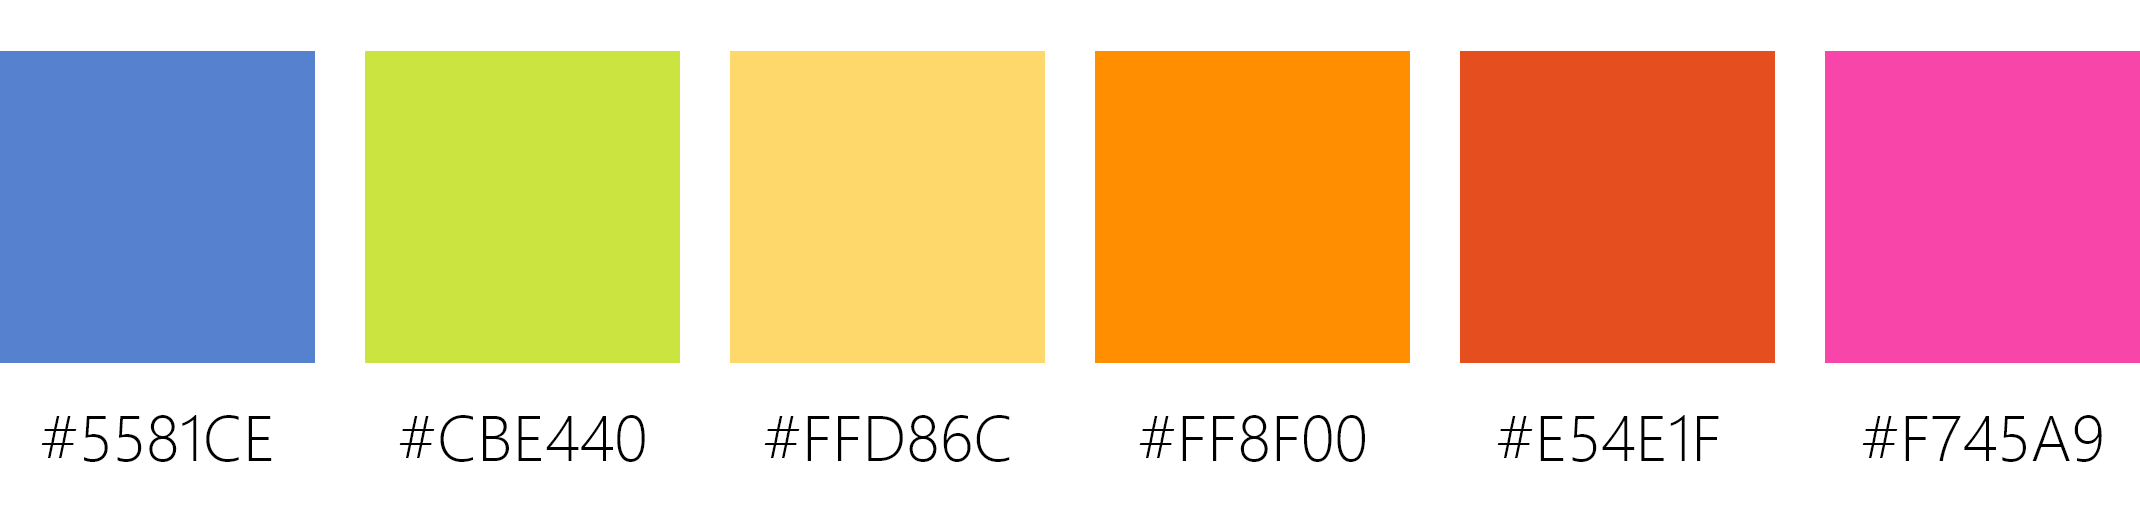
\includegraphics[width=12cm]{Farben.PNG}
\caption{Verwendete Farbpalette}
\label{fig:farben}
\end{figure}

In unserem Fall wurde der Styleguide hauptsächlich zur Dokumentation der Schrift- und Farbvorgaben genutzt. Da sich TraWo in erster Linie an Kinder richtet, war es besonders wichtig, das Farbschema bunt und ansprechend zu halten. Abbildung \ref{fig:farben} zeigt das gewählte Farbschema.

\begin{figure} [h]
\centering
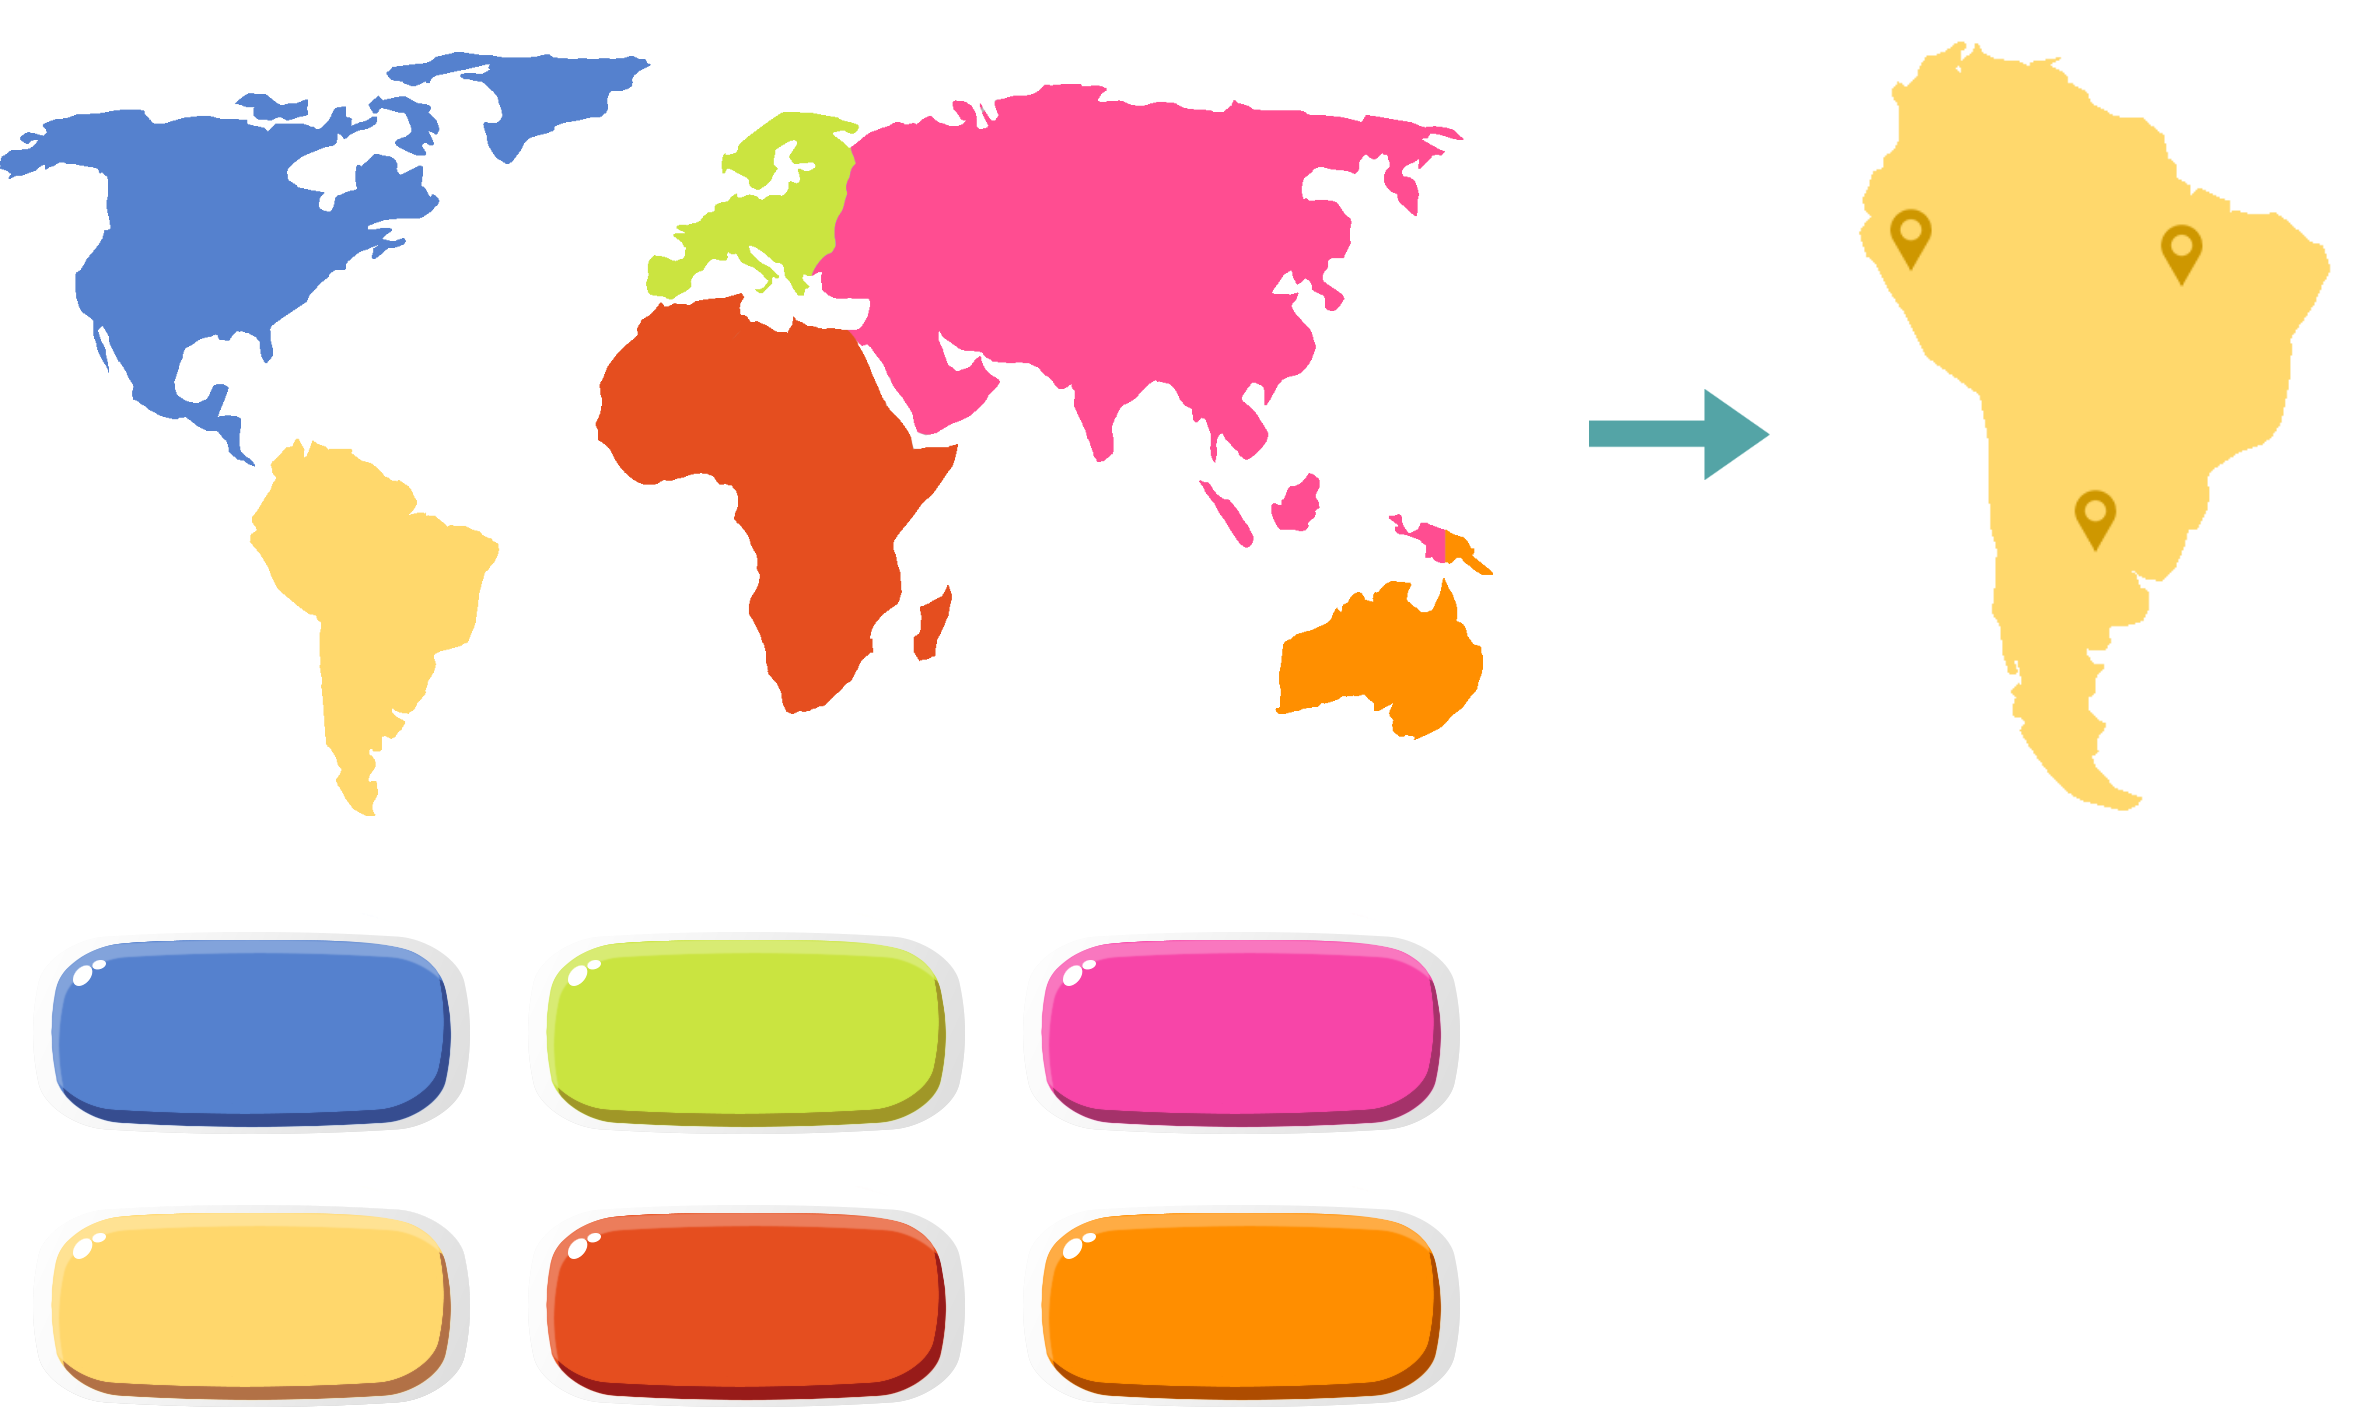
\includegraphics[width=12cm]{Map.PNG}
\caption{Landkarte und Buttons in dem genannten Farbschema}
\label{fig:map}
\end{figure}

Wie in Abbildung \ref{fig:map} zu sehen, ist wurde die oben genannte Farbpalette auf die Landkarte und die Buttons übertragen. Diese finden im Verlauf der App immer wieder an Bedeutung. Die Farben sollen vor allem zum Verständnis der Landkarte dienen und durch die Buttons zeigen, wo sich welcher Kontinent befindet. Nach der Wahl eines Kontinents soll durch Standortsymbole gekennzeichnet werden, welche Länder zur Auswahl stehen.

\subsection{Prototyp}\label{prototyp}
Ein weiterer wichtiger Schritt, der nach einem Styleguide folgt, ist die Entwicklung eines Prototyps. Abbildung \ref{fig:flowchart} zeigt, dass dieser in unserem Fall in Form eines Flowchart-Modells dargestellt wurde.

\begin{figure} [htb!]
\centering
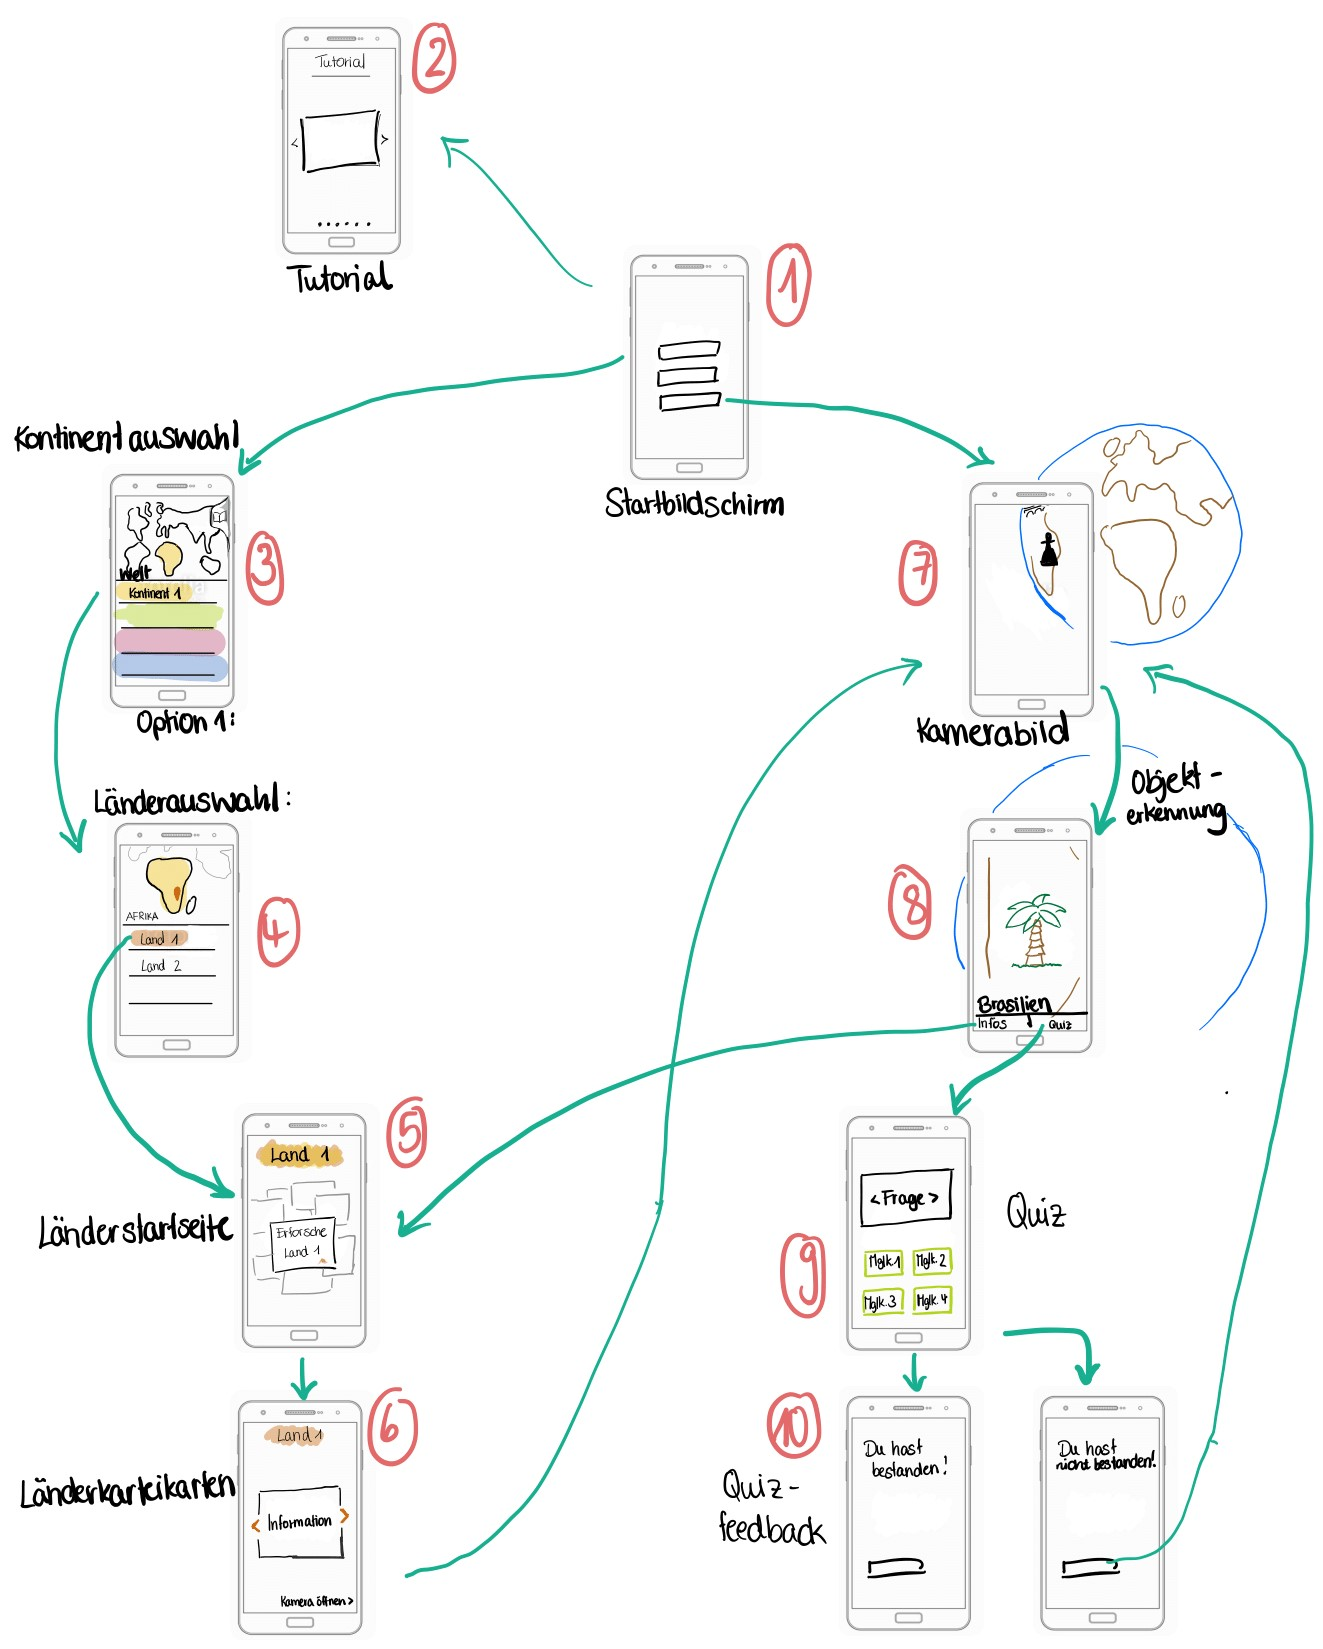
\includegraphics[width=13cm]{flowchart.JPG}
\caption{Prototyp in Form eines Flowchart-Modells}
\label{fig:flowchart}
\end{figure}

Ein Prototyp ist ein Beispiel, das als Grundlage für eine zukünftige Oberfläche dient. Es bietet die Möglichkeit, die Funktionalität des vorhandenen Designs oder Konzepts vor der Entwicklung zu testen. Somit kann vor allem Zeit gespart werden, falls Änderungswünsche während des Tests auffallen. Außerdem ist es so möglich wertvolle Rückmeldung von anderen Teammitgliedern zu erhalten, bevor das eigentliche Projekt gestartet wird. Ein einfacher Prototyp bietet außerdem mehr Freiraum bei der Entwicklung und vermeidet, dass man an kleinen Details hängen bleibt. In unserem Fall wurde der Prototyp hauptsächlich dazu genutzt einen groben Überblick für das Team zu schaffen. So hat man bereits eine Vorstellung, wie das fertige Produkt aussehen könnte und kann im Anschluss ohne Probleme mit der Entwicklung beginnen.

Der Prototyp wurde mithilfe der Anforderungen in den User Stories aus Abschnitt \ref{inhaltliche_anforderungen} erstellt. Zur Darstellung wurde sich wie bereits erwähnt für ein Flowchart-Modell entschieden. Bei einem Flowchart handelt es sich um eine grafische Darstellung des Prozesses, der die Schritte und Funktionen der einzelnen Fenster beschreibt.

Wie man in Abbildung \ref{fig:flowchart} erkennen kann, beginnt die Anwendung mit einem klassischen Hauptmenü. Von dem Menü aus ist es möglich, mit einem Tutorial zu beginnen. Dieses beschreibt in kurzen Sätzen die Funktionalität von TraWo. Ansonsten teilt sich die Anwendung in zwei Teilbereiche auf. Zum einen gelangt man in den Informationsteil, welcher von den Punkten drei bis sechs zu sehen ist. Der Nutzer entscheidet sich zunächst für einen Kontinent und wird anschließend zur Länderauswahl weitergeleitet. Von da aus gelangt er zu den Lernkarten, die die Informationen zu dem gewählten Land wiedergeben. Der zweite Teilbereich, der von den Punkten sieben bis zehn zu sehen ist, beschreibt den Augmented Reality Teil. Von hier aus ist es möglich, zum Quiz zu gelangen. Anschließend führt dieses den Nutzer je nach Ergebnis zum jeweiligen Feedback Fenster.

\section{Architekturentscheidung} \label{architekturentscheidung}
Um die inhaltlichen und grafischen Anforderungen von TraWo realisieren zu können, mussten wir uns auf eine Entwicklungsumgebung, sowie genutzte Frameworks zur Nutzung von Augmented Reality Elementen einigen. Der folgende Abschnitt beschreibt das durchgeführte Evaluationsverfahren zur Auswahl einer IDE und benötigten Tools.
\subsection{Entwicklungsumgebung}\label{entwicklungsumgebung}
Für die Entwicklungsumgebung haben sich von Anfang an zwei Favoriten herauskristallisiert. Die Wahl bestand zwischen der Gaming-Engine \textquote{Unity} und der \textquote{Android Studio} IDE. Im Folgenden werden Vor- und Nachteile der beiden Plattformen aufgelistet.

Bei erster Betrachtung liegt die Wahl der Entwicklungsumgebung Android Studio für die Entwicklung einer Android Applikation nahe. Die Umgebung ist speziell für die klassische mobile Appentwicklung prädestiniert und soll den Entwickler dabei unterstützen, eine native Android-Applikation zu erstellen. Grundsätzlich bietet Android Studio auch einige Schnittstellen zu Augmented Reality Frameworks, wie beispielsweise \textquote{ARCore} an. Da die meisten Teammitglieder wenig bis keine Erfahrung mit der Umgebung haben, wäre es zudem ein aufschlussreiches Erlebnis, diese IDE näher kennenzulernen.

Ein größeres Problem hingegen, entsteht durch das Fehlen einer integrierten 3D-Engine in Android Studio. Dadurch ist es nicht ohne Weiteres möglich, 3D-Objekte auf dem Handybildschirm zu rendern, was jedoch eine der Hauptanforderungen für die Lernapplikation darstellt. Diese Möglichkeit wäre dennoch gegeben, wenn man externe Tools wie \textquote{OpenGL} verwendet. Aus Recherchen zeigt sich jedoch, dass der Umgang damit nicht besonders einsteigerfreundlich und somit mit hohem Aufwand verbunden ist.

Der Gegenkandidat Unity ist zunächst eher aus der Videospielentwicklung bekannt. Bereits im dritten Semester durften wir alle im Fach \textquote{Software Engineering} ein Spiel mit der Engine programmieren. Damit hätte jeder aus der Gruppe zumindest eine gewisse Grunderfahrung mit der Umgebung. Auch wenn es sich zunächst kontraintuitiv anhört, Unity für eine Android-App zu benutzen, bei der es sich nicht um einen 2D-Platformer handelt, so gibt es einige Punkte, die überzeugender Weise dafür sprechen.

Grundsätzlich stellt Unity die einfache Möglichkeit bereit, die geschriebenen Skripte in eine .apk-Datei über ein integriertes Software Development Kit (SDK) umzuwandeln. Das ermöglicht uns, die für uns bequeme Programmiersprache C\# zu nutzen und gleichzeitig problemlos eine auf dem Smartphone laufende Anwendung zu erzeugen. Gute Schnittstellen zu diversen AR-Frameworks wie \textquote{AR-Core} oder \textquote{Vuforia} sind vorhanden und lassen sich leicht konfigurieren. Unitys interne 3D-Enginge ermöglicht außerdem eine aufwandslose Anzeige von Augmented Reality Inhalten. Aus der eigenen Erfahrung zeigt sich allerdings, dass Unity nicht vorwiegend für eine gestaltungsorientierte Entwicklung geeignet ist. Eventuell müsste man beim Erstellen der GUI für TraWo auf Kompromisse eingehen.

Das Team war zunächst eher dazu geneigt, mit Android Studio zu arbeiten. Auch wenn auf dem Papier Unity einem Entwickler mit der internen 3D-Engine scheinbar deutlich mehr abzunehmen scheint, hat sich für uns die Arbeit mit dem nativen Appentwickler Studio doch aufregender angehört. Bevor wir aber eine Entscheidung fällen konnten, mussten wir erst überprüfen, ob es ein favorisiertes AR-Framework gibt, welches vielleicht in Kombination mit einer der beiden IDEs als besonders erfolgreich gilt.

Alternativen wie Xamarin oder Flutter kamen für unsere Entwicklung hauptsächlich aufgrund von mangelnden Schnittstellen zu externen Frameworks nicht in Frage.
\subsection{Mustererkennung}
Das Ziel des AR-Frameworks ist es, mit Hilfe der Kamera des genutzen Smartphones, ein vorher definiertes Muster zu erkennen und eine darauf abgestimmte Reaktion abzugeben. Neben allgemeinen Erfahrungsberichten aus diversen Foren, auf die wir uns berufen haben, wurden von uns vier Kriterien aufgestellt, anhand derer wir verschiedene Framewoks miteinander verglichen haben:
\begin{itemize}
\item Tracking Stabilität
\item Dokumentation
\item Aktiver Community Support
\item Markerless Tracking Option
\end{itemize}
Die Tracking Stabilität ist ein allgemeines Qualitätssiegel dafür, wie gut die Mustererkennung des Systems funktioniert. Anzeichen dafür sind unter anderem, wie gut die Umweltbedingungen wie beispielsweise die Beleuchtung sein müssen, damit das Muster erkannt wird. Sollte diese Bewertung unterdurchschnittlich schlecht sein, käme das Framework nicht in Frage.
Um die Einarbeitung möglichst angenehm gestalten zu können, sollte das Framework über eine verständliche Dokumentation verfügen.
Falls im Laufe der Entwicklung ungeklärte Fragen auftauchen sollten, sind aktive Nutzerforen oft sogar von größerem Vorteil als die offizielle Dokumentation selbst. 

Grundsätzlich gibt es zwei Arten von Mustererkennung: Die \textquote{markerbasierte} und die \textquote{markerlose}. Wie bereits in Abschnitt \ref{projektziel} angedeutet, ist es unser Ziel, festgelegte Marker zu nutzen. Die Funktionalität dahinter wird nachher in Abschnitt \ref{einbindung_mustererkennung} näher beschrieben. Dennoch wollten wir uns die alternative \textquote{markerlose} Musterkennung, welche sich mehr auf einen Kontext in der Umgebung als ein bestimmtes Muster konzentriert, für eine eventuelle Änderung unserer Herangehensweise offen lassen.

{
\centering
\begin{tabular}{|c|c|c|c|c|c|}  
    \cline{2-6}
    \multicolumn{1}{c|}{} & Ar-Toolkit & Kudan SDK & MaxStAR & Wikitude SDK & Vuforia  \\
    \hline
    Tracing Stabilität & \xmark & \xmark & \cmark & \cmark & \cmark \\
    \hline
    Dokumentation & \xmark & \cmark & \xmark & \xmark & \cmark \\
    \hline
    Community Support & \xmark & \xmark & \xmark & \xmark & \cmark \\
    \hline
    Markerless Tracking & \cmark & \cmark & \cmark & \cmark & \cmark \\
    \hline
\end{tabular}
}

Nach diesen Kriterien haben wir nach verschiedenen Frameworks recherchiert und die resultierenden Ergebnisse in der obigen Tabelle zusammengefasst. Als Hauptreferenzen haben wir uns auf diverse Onlineforen mit Erfahrungsberichten zu den jeweiligen Frameworks berufen (vgl.\cite{Frameworks). 

Die meisten dieser Erweiterungen kamen jedoch aufgrund von schlechter Bewertung in der Tracking Stabilität oder einer mangelnden Anbindung zu unseren Entwicklungsumgebungen bereits nicht infrage. Ausschlaggebend bei der Recherche war letzten Endes, wie gut die Erfahrungswerte für die jeweilige Schnittstelle ausfielen. Die scheinbar beste Kombination schien aus Unity und Vuforia zu bestehen. Somit stand unsere Entscheidung fest.

\subsection{Datenhaltung und -bereitstellung}\label{datenhaltung und -bereitstellung}
Eines der großen Ziele für das Projekt ist die möglichst generische Haltung der Softwarestruktur, um leichte Ausbaufähigkeit sicherzustellen und die eventuelle Übertragung auf alternative Anwendungsfälle zu ermöglichen. Aus diesem Grund sollten appspezifische Inhalte nicht festcodiert, sondern nach Möglichkeit extern gelagert werden. Eine separate Datenbank soll dafür die Lösung bieten.

Neben einer strukturierteren Systemarchitektur, hätte die Nutzung einer Datenbank zugleich einen weiteren Vorteil: Man hat nun die Möglichkeit, Daten über die Laufzeit der Anwendung hinaus abzuspeichern. Das bedeutet, dass Informationen nach dem Schließen der App weiterhin erhalten bleiben. Somit haben wir eine Perspektive auf das Sichern von Spielfortschritt, welche vorher nicht gegeben war.

Die Verwendung einer Datenbank zur Datenhaltung und -bereitstellung stand also außer Frage. Es galt nun zu klären, wie genau sie erstellt und genutzt werden soll.

Um möglichst ressourcensparend arbeiten zu können, wurde sich schnell auf die Programmbibliothek \textquote{SQLite} zur Erstellung und Verwaltung geeinigt. Ihr Hauptvorteil ist ihr minimalistischer Aufbau. Als eines der kompaktesten Datenbanksysteme, besitzt SQLite zwar nur eine beschränkte Funktionalität für das Arbeiten mit Datenbanken, ist dafür aber für die Datenbankverwaltung vollkommen unabhängig von weiterer Software. So ist zum Beispiel, im Gegensatz zu komplexeren Bibliotheken, wie \textquote{Microsoft SQL Server}, keine weitere Serveranbindung nötig. Außerdem ist zu Unity und vielen anderen Entwicklungsumgebungen eine passende Schnittstelle vorhanden.

Die frei verfügbare Software \textquote{DB Browser for SQLite} eignet sich angemessen als graphische Benutzeroberfläche für die Arbeit direkt an der Datenbank. So lassen sich damit ganze Querys direkt ausführen, oder über Shortcuts beispielsweise Tabellen einfach erzeugen.

Die Tatsachen, dass sich SQLite denkbar einfach in die Entwicklung einbinden lässt und der geringe Speicherverbrauch des Datenbanksystems, machen die Programmbibliothek zu einem beliebten Kandidaten für die mobile Appentwicklung. Die abgeschwächte Funktionalität im Vergleich zu gewohntem SQL, sollte für uns kein Hinderungsfaktor sein, da wir davon ausgingen, keine sonderlich komplexe Datenbankstruktur aufzubauen. Für den in diesem Kontext geringen Tabellenumfang, schien es das optimale System zu sein. 

Somit standen alle zu nutzenden Technologien für das Projekt fest und es konnte mit der Realisierung angefangen werden. Bevor die eigentliche Umsetzung beschrieben wird, folgt im kommenden Abschnitt eine genau Erläuterung der Funktionsweise einiger Komponenten für eine bessere Übersicht des Projektumfangs und eines allgemeinen Verständnisses für die Arbeitsweise der entstandenen Applikation.
\chapter{Funktionsweise der Komponenten}\label{ch:funktionsweise_der_komponenten}
\section{Mustererkennung in Vuforia}
\section{Aufbau einer Unity-Applikation}
\chapter{Realisierung}\label{ch:realisierung_der_anwendung}
In den nachfolgenden Abschnitten werden alle für die Implementierung wichtigen technischen Aspekte und deren Umsetzung erläutert. Es wird einen Einblick in die Arbeitsweise mit dem AR-Framework Vuforia im Zusammenspiel mit dem Rendern von 3D Objekten gegeben. Des Weiteren wird die interne Datenhaltung, sowie die Umsetzung einzelnen Szenen in Unity beschrieben.

\section{Einbindung der Mustererkennung}\label{einbindung_mustererkennung}
In Abschnitt \ref{mustererkennung_vuforia} wurde bereits näher die internen Funktionsweise des Augmented Reality Frameworks \textquote{Vuforia} erklärt. 
Um dessen vollen Umfang in der Unity-Projektumgebung nutzen zu können, musste das entsprechende Vuforia Software Development Kit eingebunden werden.
Es beinhaltet im Wesentlichen alle Grundbausteine für die Entwicklung einer Augmented Reality App und stellt diese in Form von Unity GameObjects (vgl. Abschnitt \ref{aufbau_unity_app}) bereit. 
Dadurch sind sie genau wie herkömmliche GameObjects nutzbar und können einfach in ein bestehendes Unity-Projekt integriert werden, um dieses zu erweitern.

Ein Beispiel für einen solchen Baustein ist die AR Camera. 
Sie beinhaltet Logik, um die Hauptkamera des ausführenden Gerätes anzusteuern. 
Die Szene in der die Kamera platziert wurde, wird nun in das Kamerabild der realen Welt projiziert.
Dieser Baustein ist essentiell für die Erstellung einer Augmented Reality App. 

Auf einen weiteren essentiellen Baustein aus der Vuforia SDK wird in den nachfolgenden Unterabschnitten \ref{image_targets} und \ref{integration_image_targets} eingegangen. 

\subsection{Image Targets}\label{image_targets}
Da wir uns in der Anwendung für die markerbasierte Variante der Augmented Reality entschieden haben, benötigen wir hierzu die passenden Marker. 
Wie bereits in Abschnitt \ref{mustererkennung_vuforia} beschrieben, bietet Vuforia hier die Möglichkeit, eigene Image Targets zu verwenden. 
Da diese innerhalb der Anwendung möglichst gut erkannt werden sollen, müssen bei der Wahl der Bilder einige Qualitätskriterien beachtet werden.

Eines dieser Kriterien sind die Ecken und Kanten im Bild, welche durch die Featureextraktion beim Hochladen des Bildes berücksichtigt werden. 
Jede scharfe Ecke und Kante wird als Feature abgespeichert und dient später bei der Bilderkennung innerhalb der Anwendung als Vergleichsmerkmal. 
Je mehr dieser markanten Punkte im Bild vorhanden sind, desto leichter fällt es der Vuforia Engine das Image Target im Kamerabild der AR-Anwendung zu identifizieren (vgl. \cite{ImageTarget2018}).

Um sicherzugehen, dass aus dem gewählten Image Target viele Features extrahiert werden können, sollte das Bild hohe lokale Kontraste besitzen. Das heißt, es sollte ausreichen viele Stellen geben, an denen sehr helle Pixel neben sehr dunklen liegen. 
Hiermit ergeben sich ausgeprägte Farbunterschiede und somit schärfere Ecken und Kanten, welche als potentielle Features in Frage kommen (vgl. \cite{ImageTarget2018}).

\begin{figure} [h]
\centering
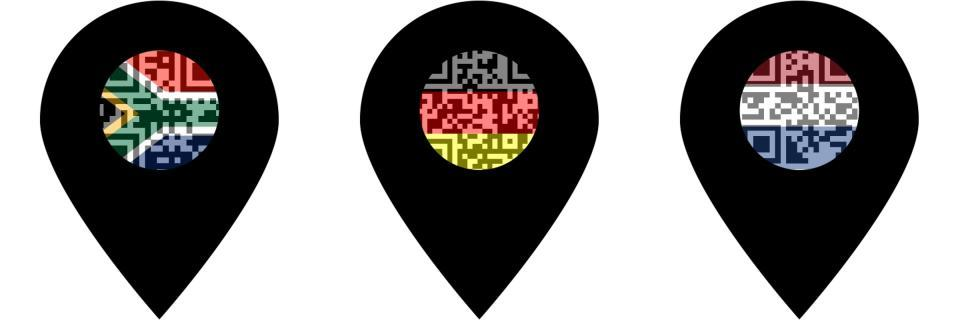
\includegraphics[width=12cm]{Image_Targets.jpg}
\caption{Beispiele der verwendeten Image Targets}
\label{fig:image_targets}
\end{figure}

In Abbildung \ref{fig:image_targets} sind die finalen Image Targets der beschriebenen Anwendung zu sehen.
Die Grundform der Targets stellt die heutzutage sehr häufig genutzte Form des Standortsymbols dar.
Wir wählten die Form um die Erdkundethematik der Anwendung zu unterstreichen.
Diese werden in der Praxis auf einem Globus platziert und jedes Target repräsentiert ein Land.
Um die Verbindung zu dem jeweiligem Land erkenntlich zu machen, ist Flagge des Landes in das Standortsymbol integriert. 
Somit ist jedes Image Target einzigartig und lässt sich von den anderen unterscheiden. 
Der Nutzer der Anwendung kann jetzt erkennen, welches Image Target zu welchem Land gehört und kann sich gleichzeitig die Flaggen der Länder einprägen. 

Nun sind zwar alle Targets einzigartig und können in manchen Fällen sehr gut unterschieden werden, jedoch ist das noch nicht ausreichend um bei der Targeterkennung befriedigende Ergebnisse zu erhalten. 
Bei der Merkmalsextraktion werden die Bilder in Graustufen umgewandelt und verlieren somit jegliche Farbinformationen. Dies kann beispielsweise bei den Flaggen von Deutschland und den Niederlanden zu Schwierigkeiten in der Unterscheidung führen, da sie aus den exakt gleichen Formen bestehen. 
Die Ecken- und Kantenmerkmale wären damit sehr ähnlich. 
Um dieses Problem zu lösen, hinterlegten wir jede Flagge mit einem individuellem QR-Code. 
Dieser ist leicht transparent, bringt aber dennoch mehr Kontrast in das Bild. 
Somit können selbst aus den einfach geformten Flaggen genügend eindeutige Merkmale erzeugt werden.

Diese Art der Image Targets resultiert in der Vuforia Engine in einer Fünf-Sterne Erkennungsrate.

\subsection{Integration der Image Targets}\label{integration_image_targets}
Nachdem nun alle fertigen Image Targets über das in Abschnitt \ref{mustererkennung_vuforia} beschriebene Target Management System geladen wurden, müssen diese in die Anwendungsumgebung integriert werden.
Hierzu wird aus der Weboberfläche eine Datenbank erzeugt, die alle Targets enthält. 
Anschließend wird sie als \textquote{.unitypackage}-Datei heruntergeladen und kann in das bestehende Unityprojekt importiert werden.

Um nun die einzelnen Image Targets innerhalb der Anwendung nutzbar zu machen, wurde zunächst eine dedizierte Szene erstellt. 
In dieser Szene befindet sich zuerst einmal die AR Camera, welche in Abschnitt \ref{einbindung_mustererkennung} beschrieben ist. 
Des Weiteren wird für jedes vorhandene Land das passende Target benötigt.
Ein Image Target wird in Form eines GameObjects in die Szene geladen.
Es ist ein spezieller Typ von GameObject, welcher von der Vuforia-SDK mitgeliefert wird und bereits vordefinierte Logik in Form von Komponenten enthält.
Ein Beispiel hierfür ist die Scriptkomponente \textquote{Image Target Behaviour}, welche die Kommunikation mit der Image Target Datenbank regelt. 
Sie bietet die Möglichkeit, zwischen allen importierten Datenbanken und den darin enthaltenen Image Targets zu wählen.
Wählt man jetzt beim ersten GameObject das Target des Landes Indien, so erscheint an der Stelle des vorher leeren Objekts, das erstellte Image Target für genau dieses Land.
Dieser Vorgang muss nun für alle restlichen Länder wiederholen, damit alle in der Szene enthalten sind.

Wenn nun die fertige Szene gestartet wird, öffnet sich zunächst die Kamera des ausführenden Geräts.
Im Hintergrund wird das Kamerabild ständig untersucht und geprüft, ob sich eines der in der Szene liegenden Image Targets im Sichtfeld befindet. Im Falle einer Bilderkennung können unterschiedliche Aktionen ausgeführt werden, welche in Abschnitt \ref{einbindung_3D_objekte} genauer beschrieben werden.

\section{Verwendung von 3D Objekten}\label{verwendung_3d_objekte}
Die in der Anwendung verwendeten 3D Objekte liegen im \textquote{object}-Format vor, welches durch die Dateiendung \textquote{.obj} gekennzeichnet ist. 
Dem Dateiformat liegt das polygonale Modell zugrunde, das 3D Objekte als Zusammensetzung von Polygonen, die wiederum aus durch Kanten verbundenen Koordinaten bestehen, definiert. 
Die geläufigsten so entstehenden Polygonnetze sind Dreiecksnetze und Vierecksnetze.

In einer  \textquote{.obj}-Datei sind somit die Koordinaten von Punkten im dreidimensionalen Raum definiert, welche über Kantendefinitionen zu Flächen verbunden werden. 
Um 3D Objekte realistisch erscheinen zu lassen, findet der Prozess des sogenannten \textquote{Texture Mappings} statt, in welchem eine Textur im Bildformat über ein 3D Objekt gelegt wird. 
Auf Codebasis wird dies realisiert, indem in der \textquote{.obj}-Datei zweidimensionale Texturkoordinaten für eine vorhandene Textur definiert und bestimmten Punktkoordinaten des Objekts zugewiesen werden.

Primitive 3D Objekte, die aus wenigen Polygonen bestehen, können somit leicht selbst erstellt werden, während die Erstellung von komplexeren Objekten und zugehörigen Texturen mehr Zeitaufwand erfordert. 
Da dieser Zeitaufwand nicht in den zeitlichen Rahmen dieses IT Projektes gepasst hat, haben wir uns dafür entschieden, kostenlose 3D Objekte mit zugehörigen Texturen von verschiedenen Anbietern aus dem Internet zu verwenden, welche im folgenden aufgelistet sind.

\begin{itemize}
\item https://www.turbosquid.com/
\item https://www.cgtrader.com/
\item https://free3d.com/
\end{itemize}

Wie bereits in Abschnitt \ref{projektziel} erwähnt, sollen die in der App enthaltenen Länder durch passende 3D Objekte repräsentiert werden, welche auf das erkannte Image Target eines Landes gerendert werden. 
Die folgende Auflistung zeigt die gewählten 3D Objekte für ihre zugehörigen Länder, gegliedert in Kontinente. Diese sind bildlich auch im Anhang dargestellt.

\textbf{3D Objekte für Afrika:}
\begin{itemize}
\item Kongo: Affe
\item Südafrika: Elefant
\item Ägypten: Pyramide
\end{itemize}

\textbf{3D Objekte für Europa:}
\begin{itemize}
\item Deutschland: Brandenburger Tor	
\item Frankreich: Eiffelturm
\item Niederlande: Windmühle
\end{itemize}

\textbf{3D Objekte für Nordamerika:}
\begin{itemize}
\item Kanada: Hirsch
\item USA: Empire State Building
\item Mexico: Maya Tempel
\end{itemize}

\textbf{3D Objekte für Südamerika:}
\begin{itemize}
\item Brasilien: Palmenwald
\item Argentinien: Pinguine
\item Peru: Machu Picchu
\end{itemize}

\textbf{3D Objekte für Asien:}
\begin{itemize}
\item Indien: Taj Mahal
\item Malaysia: Petrona Towers
\item Japan: Tempel
\end{itemize}

Die Einbindung dieser 3D Objekte und die dazu nötige Vorverarbeitung dieser werden in den folgenden Abschnitten beschrieben.
\subsection{Vorverarbeitung}
Die Vorverarbeitung der 3D Objekte wurde mit dem kostenlosen Grafikprogramm \textquote{Blender} realisiert, welches einen großen Funktionsumfang für die Bearbeitung und Erstellung von 3D Körpern bietet. 

Die vorherige Bearbeitung der 3D Objekte war hauptsächlich aus zwei Gründen nötig. 
Zum Einen erleichterte sie die Einbindung der Objekte, da die aus unterschiedlichen Quellen stammenden 3D Objekte meist sehr groß skaliert und rotiert waren.
Durch einfache Transformationsoperationen konnten diese Objekte somit auf eine einheitliche Größe und Ausrichtung normalisiert werden, wodurch die aufwendigere Bearbeitung in Unity nicht mehr nötig war.

Ein weiterer Anwendungsfall für die nötige Vorverarbeitung der 3D Objekte in Blender war die nötige Reduktion der Polygonzahl der Objekte. 
Die aus dem Internet stammenden Körper wiesen eine sehr hohe Polygonzahl auf und waren dadurch sehr hoch aufgelöst, was zu einer größeren Dateigröße und somit einer Belastung des Anwendungsspeichers führen würde. 
Eine solch hohe Auflösung war in unserem Anwendungsfall nicht nötig, da die 3D Objekte auf dem Globus sehr klein skaliert angezeigt werden und die gegebenen Genauigkeiten somit nicht auffallen würden. 
Um Speicherplatz innerhalb der App zu sparen wurde die Polygonzahl und damit die Dateigröße der 3D Objekte mithilfe von Blender um das zehnfache verringert, bevor diese in der App eingebunden wurden.

Die Veränderung der Polygonzahl wird durch Grafiken \ref{fig:elefant_viele_polygone} und \ref{fig:elefant_wenig_polygone} dargestellt.

\begin{figure}[!htb]
\minipage{0.48\textwidth}
  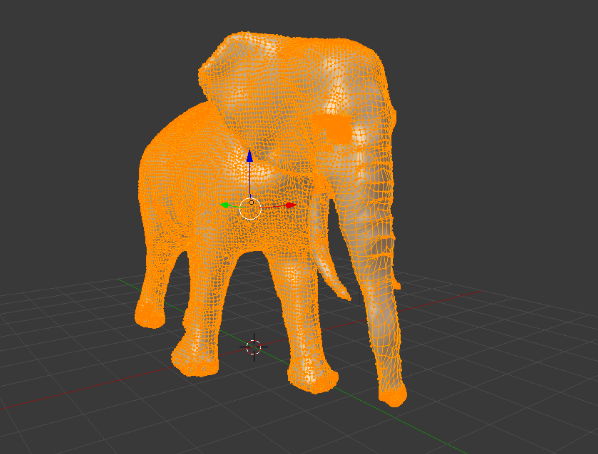
\includegraphics[width=\linewidth]{elefant_viele_polygone.png}
  \caption{Polygonnetz vor Bearbeitung}\label{fig:elefant_viele_polygone}
\endminipage\hfill
\minipage{0.48\textwidth}
  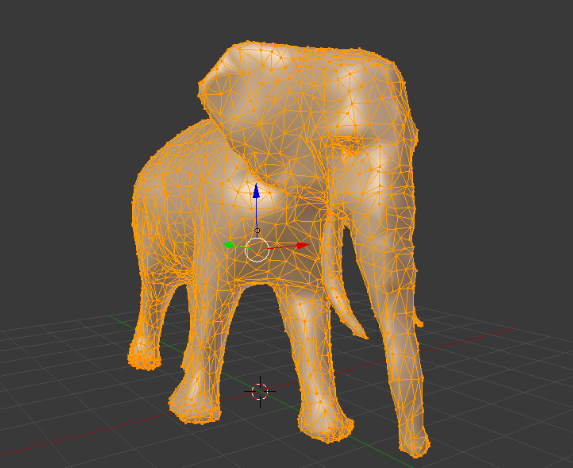
\includegraphics[width=\linewidth]{elefant_wenig_polygone.png}
  \caption{Polygonnetz nach Bearbeitung}\label{fig:elefant_wenig_polygone}
\endminipage\hfill
\end{figure}

Aus Grafik \ref{fig:elefant_wenig_polygone} geht hervor, dass sich die Gestalt des 3D Objektes trotz verringerter Polygonzahl kaum verändert und der Prozess der Polygonreduktion somit zu einem nicht merklichen Genauigkeitsverlust führt.
\subsection{Einbindung der 3D Objekte in Unity}\label{einbindung_3D_objekte}
Der Zugriff auf die ausgewählten 3D Objekte innerhalb des Unity-Entwicklungsoberfläche, sowie der Applikation wird ermöglicht, indem die Objekte im Projektpfad als Ressourcen abgelegt werden, welche beim Bauen der Applikation auf das Endgerät mit übertragen werden. 

Wie in Abschnitt \ref{projektziel} beschrieben, soll ein 3D Objekt nur bei der Erkennung des ihm zugeordneten Landes angezeigt werden.
Um dies zu realisieren, werden die 3D Objekte in der Entwicklungsoberfläche als Kind-Objekte der in Abschnitt \ref{integration_image_targets} beschriebenen Image-Targets angelegt.
Das Verhalten dieser Vuforia-Elemente wird durch das \textquote{DefaultTrackableEvent-Handler}-Skript bestimmt, welches den Elementen standardmäßig beigefügt ist. 
Bei der Feuerung des \textquote{OnTrackableFound}-Events, das heißt der Erkennung eines Image-Targets, werden die diesem untergeordneten, renderbaren Kindelemente mithilfe der von Unity bereitgestellten \textquote{Renderer}-Klasse automatisch gerendert.

Das beschriebene \textquote{DefaultTrackable-EventHandler}-Skript kann nach Belieben bearbeitet werden, um ein besonderes, durch den Benutzer gewünschtes Verhalten hervorzurufen.
In unserem Fall wurde das \textquote{OnTrackable-Found}-Event so erweitert, dass zusätzlich zu dem 3D Objekt noch zwei Buttons angezeigt werden, mit welchen der User interagieren kann.

\section{Verwaltung der Daten}
Im Abschnitt \ref{datenhaltung und -bereitstellung} wurde bereits das geplante Vorgehen für die Erstellung und Verwaltung einer Datenbank mit \textquote{SQLite} erläutert. Der folgende Absatz beschreibt nun das resultierende Datenbankmodell, sowie die Interaktion der Applikation mit den gespeicherten Informationen.
\subsection{Datenbankentwurf}\label{datenbankentwurf}
Aus der Planung haben sich insgesamt fünf Tabellen entwickelt. Die Tabellen \textquote{Information}, \textquote{Question} und \textquote{Answer} dienen hauptsächlich der Speicherung von austauschbaren Inhalten für den Informations- und Lernteil von TraWo. Hier liegen die Informationen, Fragen und Antworten, auf die der Spieler bei der Nutzung der App trifft. Die Tabellen \textquote{Country} und \textquote{Continent} sind eher als Zuweisungstabellen zu betrachten und spielen für die Codierung der Spiels eine große Rolle.

\begin{figure} [h]
\centering
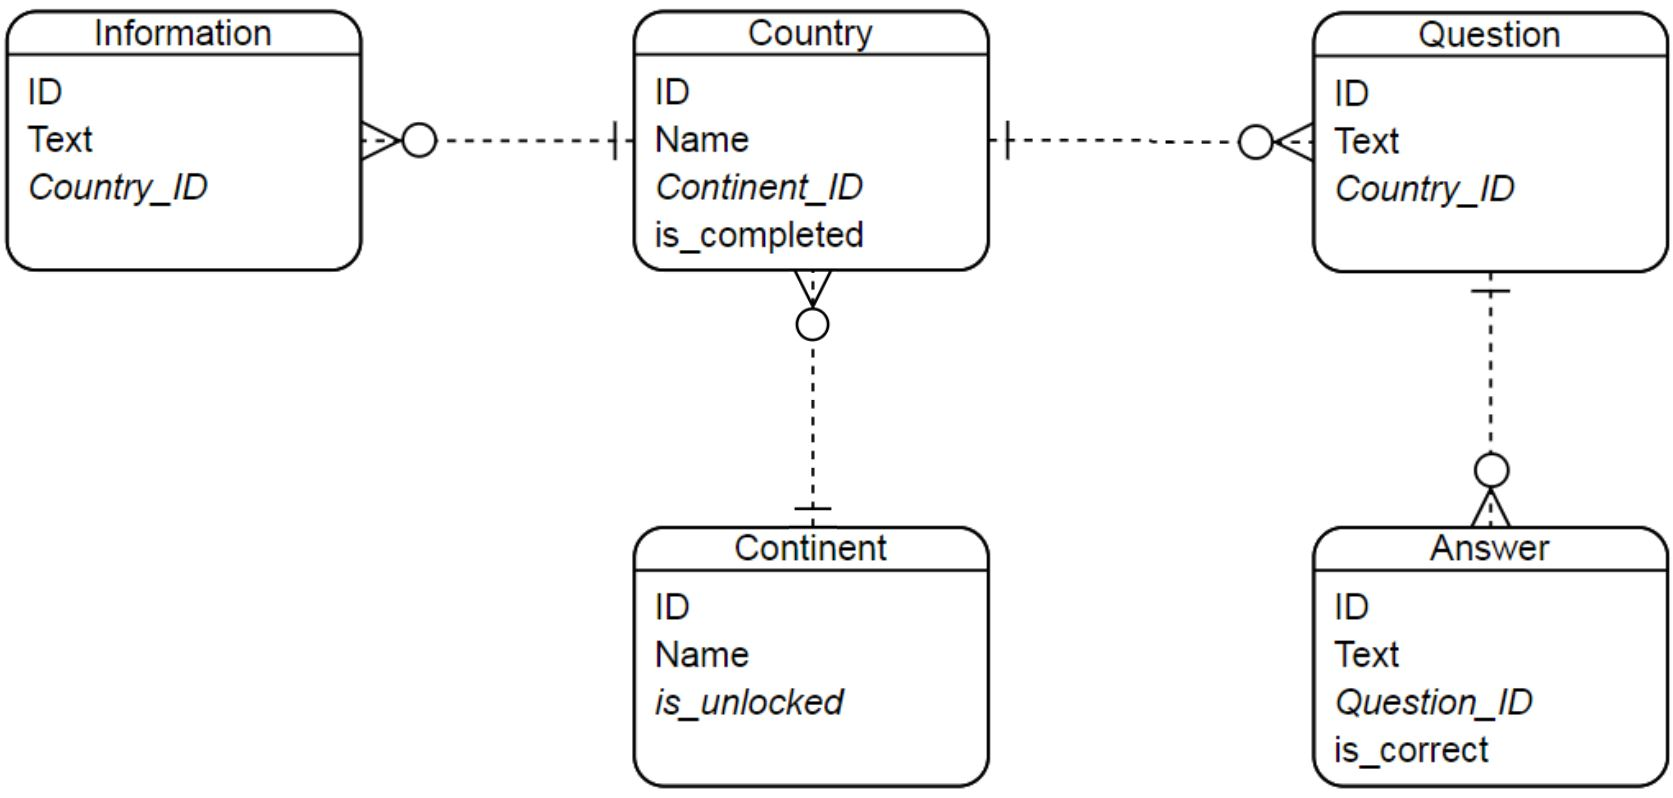
\includegraphics[width=12cm]{Datenbankentwurf.jpg}
\caption{Datenbankentwurf}
\label{fig:db_model}
\end{figure}

Die Grafik \ref{fig:db_model} stellt das Datenbankmodell in der Martin-Notation dar. Die, auch Krähenfußnotation genannte, Darstellung zu \textit{Entity-Relationship}-Modellen eignet sich, neben Alternativen wie der Chen-Notation, um eine visuelle Repräsentation von Datenbankentwürfen darzustellen. 

Hierbei sollen die semantischen Zusammenhänge zwischen einzelnen Tabellen in Form von Entitäten aufgezeigt werden, die als Rechtecke abgebildet sind. Neben dem Namen des Entitätstypen enthalten sie noch Attribute, welche die Spaltennamen darstellen. Fremdschlüssel sind als Verweis auf andere Tabellen in Form von referenzierten IDs ebenfalls enthalten. Die Beziehungen der Entitäten stellen die Verbindungslinien dar. Diese geben gleichzeitig über Symbole an den Enden Aufschluss über die Kardinalität der Entität in der gegebenen Relation. Ein perpendikular zur Verbindungslinie verlaufender Strich steht für \textquote{eins}, der namensgebende Krähenfuß steht für \textquote{mehrere}.

Die im Diagramm gezeigten Beziehungen Beziehungen lassen sich nun wie folgt lesen:
\begin{itemize}
\item Ein Land enthält mehrere Informationen
\item Ein Land enthält mehrere Fragen
\item Ein Kontinent enthält mehrere Länder
\item Eine Frage enthält mehrere Antworten
\end{itemize}

Die Attribute bestehen pro Eintrag zunächst immer aus einer eindeutigen ID. Tabellen mit apprelevanten Inhalten besitzen einen Text, in dem der zugehörige Content gespeichert ist. Zuweisungstabellen besitzen einen Namen. Steht die Tabelle in einer 1:n-Beziehung, so hat die n-seitige Tabelle eine Referenz auf die konkrete, ihr zugehörige Instanz. Beispielsweise hat eine Antwort immer eine passende \textit{Question\_ID}, damit sie der passenden Frage zugeordnet werden kann. Zuletzt besitzen drei Tabellen einen boolschen-Wert, der wahr oder falsch sein kann. Für die Antworten lässt sich damit bestimmen, ob eine im Quiz angezeigte Antwort richtig oder falsch ist. Für die Länder und Kontinente wird der Wert als Zustandsindikator verwendet. Somit lassen könnte man kennzeichnen, ob für ein Land alle Quizze gelöst wurden, beziehungsweise ob ein Kontinent freigeschaltet und somit spielbar ist.

Das Prinzip ähnelt einem UML-Diagramm für Softwarearchitekturen aus der Softwareentwicklung. Zum einen kann das die Lesbarkeit für alle beteiligten Entwickler erhöhen, selbst wenn sie ansonsten keinen Bezug zu der Datenbankentwicklung hätten, zum anderen kann es sich auch als ein geeigneter Bauplan für die grundlegende Klassenstruktur eines Projektes eignen. Da wir unseren Datenbankentwurf fertig gestellt hatten, bevor wir mit der Ausimplementierung des Codes angefangen haben, ist uns dieser \textit{Model-First Approach} sehr entgegengekommen.

Im nachfolgenden Abschnitt wird näher auf die technische Umsetzung der Datenbank und deren Einbindung in Unity eingegangen.

\subsection{Zugriff auf Datenbankinhalte}\label{zugriff_datenbank}
Unity ist durch Nutzung der \textquote{Mono.Data.SQLite.dll} in der Lage, SQlite-Befehle auszuführen. Dadurch lassen sich Methoden schreiben, die bei Bedarf mit einer Datenbank interagieren.

Jede dieser Methoden braucht dabei eine Datenbankverbindung und einen ausführbaren SQLite-Befehl. Da sich die Verbindung immer auf die selbe Datenbank bezieht, ist sie als ein konstanter String mit einem relativen Systempfad festgeschrieben. Jeder Aufruf der Datenbank muss diese Verbindung öffnen, und nach Ende des Prozesses wieder schließen. Durch den relativen Pfad wird sichergestellt, dass die Kommunikation mit der Datenbank spezifisch für jedes individuelle Gerät ist. Der Befehl ist dagegen einzigartig für jede Funktion, und erfüllt einen bestimmen Zweck.

Die meisten Methoden sind Lesefunktionen, und sollen somit Inhalte aus der Datenbank auslesen, damit die Anwendung diese verarbeiten kann. Beispielsweise sollen beim Start eines Quiz die möglichen Antworten geladen werden. Die aufgerufene Methode führt nun ein entsprechendes Skript aus und speichert das von der Datenbank kommende Ergebnis in einem \textquote{SqliteDataReader}-Objekt ab. Durch das Iterieren über das Objekt können die Daten konvertiert und weiterverarbeitet werden. Nach diesem Prinzip läuft jeder Datenbankzugriff ab. Doch wie können die Daten konvertiert und nutzbar gemacht werden?

Basierend auf dem Datenbankmodell wurden entsprechende Entitäten im Unity-Skript angelegt. Dadurch hat jede Tabelle eine äquivalente C\#-Klasse mit allen dazugehörigen Attributen und Referenzen, die die Datenbankstruktur als Klassenstruktur widerspiegeln. Die beim Auslesen gewonnenen Daten können somit als Objekte weitergereicht und verarbeitet werden. 

Da es sich im gegebenen Modell um eine relativ einfache Struktur handelt, wurde auf die Nutzung von Frameworks wie \textquote{Entity-Framework} verzichtet. Mit der Hilfe von solchen Frameworks, könnte man automatisiert nach dem \textit{Model-First} beziehungsweise \textit{Code-First Approach} passende C\#-Klassen, respektive eine passende Datenbankstruktur erzeugen lassen. Die manuelle Herangehensweise ist allerdings ressourcensparender und gestaltet sich bei kleineren Projekten in der Regel einfacher und übersichtlicher.

Neben den Lesemethoden, wird beim Start von TraWo einmalig ein SQL-Skript zum Erzeugen und Befüllen der eigentlichen Datenbank mit festgeschriebenem Inhalt nach dem obigen Modell ausgeführt. Die Datenbank wird dann lokal auf dem Anwendungsgerät in einer .db-Datei gespeichert und ist zugriffsbereit. 

\section{Realisierung der Anwendung in Unity}\label{realisierung_unity}
Im Abschnitt \ref{aufbau_unity_app} des Berichts, wurde bereits der generelle Aufbau einer Unity-Anwendung erläutert.
Wie unsere Anwendung nun aufgegliedert ist wird im nachfolgenden Teil behandelt.

Insgesamt besteht die Applikation aus neun Szenen, welche in Abschnitt \ref{prototyp} in Form eines Flowcharts vorgestellt wurden.
Des weiteren findet sich in Abschnitt \ref{einblick} des Anhang ein Gesamtüberblick über alle finalen Szenen der Applikation.
Angefangen mit der Menüszene, von der aus man entweder in die Onboarding-Szene für das Tutorial, den Spiel- oder den Informationsteil gelangt. 
Der Spiel- und der Informationsteil setzen sich wiederum aus eigenen Szenen zusammen, zu welchen in den nächsten beiden Abschnitten mehr Informationen folgen. 
Die Abbildung \ref{fig:scenegraph} gibt einen gesamten Überblick über die vorhandenen Szenen und deren Übergänge.

\begin{figure} [h]
\centering
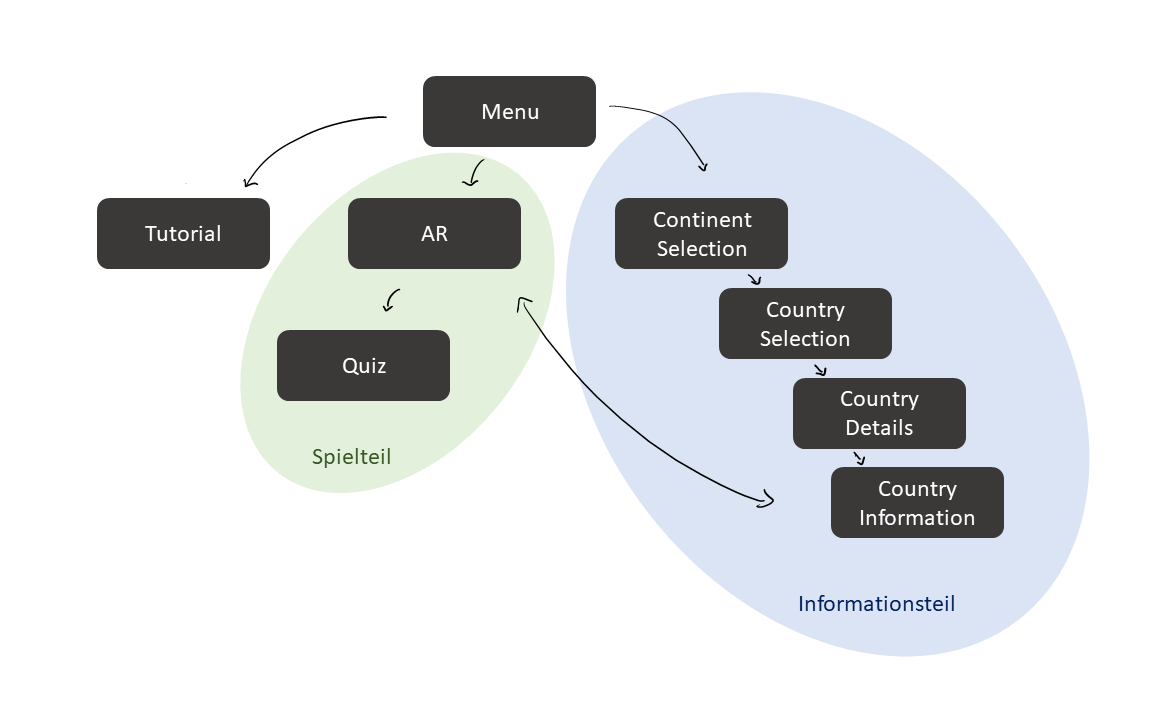
\includegraphics[width=14cm]{Szenenuebersicht.PNG}
\caption{Szenengraph der gesamten Anwendung}
\label{fig:scenegraph}
\end{figure}

Jede Szene besteht aus verschiedenen UI-Elementen, wie beispielsweise Buttons und Textflächen. Je nachdem ob diese mit dynamischer Interaktivität versehen sind, besitzen sie ihr eigenes C\#-Script, welches sich um individuelle Anpassungen kümmert.

\subsection{Informationsbereich}
Der Informationsteil besteht aus vier Einzelszenen. 
In den ersten beiden wählt der Nutzer einen Kontinent und daraufhin ein Land, über das er etwas erfahren möchte.
Anschließend folgt eine Zwischenszene, welche als Vorschau für das gewählte Land dient und danach startet die eigentliche Informationsszene. 

Um den ganzen Bereich dynamisch zu halten, befinden sich in den Szenen nur Dummyobjekte, welche noch nicht mit Texten befüllt sind. Das heißt, dass beispielsweise die Kontinentauswahl vorerst nur leere Buttons und die Informationsszene leere Informationsfelder enthält.
Durch die in Abschnitt \ref{zugriff_datenbank} beschriebene Datenbankschnittstelle, werden diese nun beim Laden der Szene mit Inhalten befüllt. 
In diesem Zuge werden die leeren Auswahlbuttons in der Kontinent- und der Länderszene, dem Styleguide entsprechend unterschiedlich eingefärbt. Und die leeren Informationsfelder werden mit hilfreichen Fakten beschrieben.
Dies wird im Folgenden am Beispiel der Informationsszene verdeutlicht.

Zunächst werfen wir einen Blick auf die vorangehende Szene, in welcher ein Land gewählt wird. 
Beim Tippen auf eines der wählbaren Länder wird das \textquote{Behaviour-Script} dieser Szene aufgerufen, in dem sich ein \textquote{onClick-Event} befindet. 
In diesem wird der Inhalt des angeklickten Objekts, also der Name des jeweiligen Landes, ausgelesen und zwischengespeichert. 
Nun kann er als Parameter an die Datenbankfunktion weitergereicht werden, welche für das Laden der Informationen eines Landes zuständig ist. 
Die daraus resultierenden Daten stehen nun in der darauffolgenden Informationsszene in Form einer Liste zur Verfügung.
Beim Laden der Szene wird deren Behaviour-Script geladen und die darin enthaltene \textquote{Start}-Methode ausgeführt. Diese dient zur Initialisierung der Szene und verarbeitet die vorher erlangten Daten.
Es wird mithilfe einer Schleife über die zwischengespeicherten Informationstexte iteriert, und für jeden Textblock in der Szene wird das jeweilige Textattribut ersetzt.
Die GameObjects der Textblöcke für die einzelnen Informationen müssen hierfür vorher im Script referenziert werden, damit darauf zugegriffen werden kann.

\begin{figure} [h]
\centering
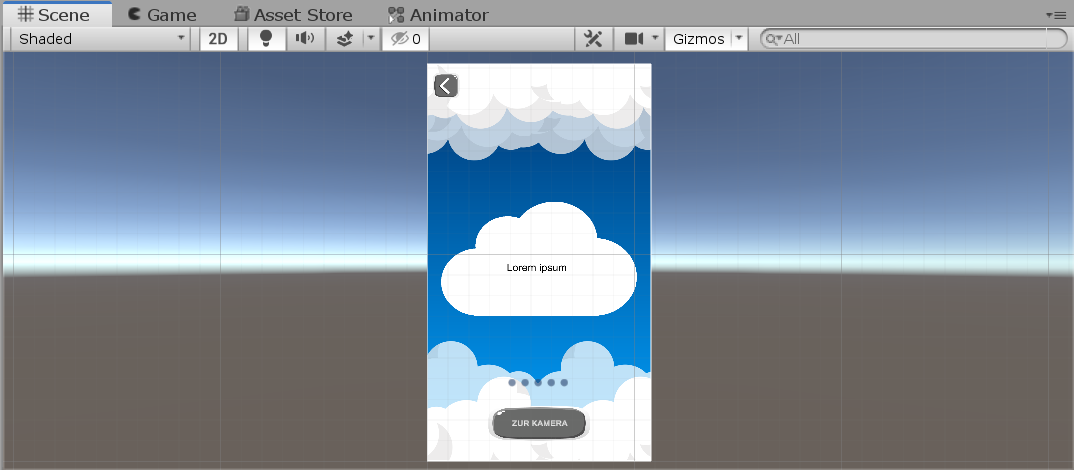
\includegraphics[width=14cm]{Informationsszene.PNG}
\caption{Initialer Status der Informationsszene}
\label{fig:infoscene}
\end{figure}
Die genannten Informationstexte sind in einzelne Elemente aufgeteilt, welche sich innerhalb eines horizontal scrollbaren Containers befinden. 
Es ist immer nur ein Informationselement sichtbar und mithilfe einer Wischgeste kann der Nutzer zur nächsten Information wechseln.
Die in Abbildung \ref{fig:infoscene} erkennbare kleine Anzeige unterhalb des Informationsfeldes zeigt an, welches der fünf Informationsfelder gerade gezeigt wird.
Diese Anzeige wird auch \textquote{Pagination} genannt, da sich die einzelnen Elemente wie scrollbare Seiten verhalten.
Für die Scrollbox und die Pagination musste ein externes Unity Packet installiert und importiert werden, welches beide Funktionen in Form neuer GameObjects hinzufügt.
Die Szenenhierarchie der Informationsszene besteht nun aus der Kamera, einem Szenenscript und einem UI-Container. 
Innerhalb des Containers befinden sich die beiden eben genannten Komponenten, sowie ein Button, um in die AR-Szene zu gelangen.

\subsection{Quizbereich}
Ein ähnliches Grundprinzip wurde bei der Umsetzung der Quizszene verfolgt.
Wie in Abbildung \ref{fig:quizscene} zu sehen, wurde die Benutzeroberfläche ebenfalls mit GameObjects vormodelliert, sodass deren Textinhalte aus Platzhalterwerten bestehen.

\begin{figure} [h]
\centering
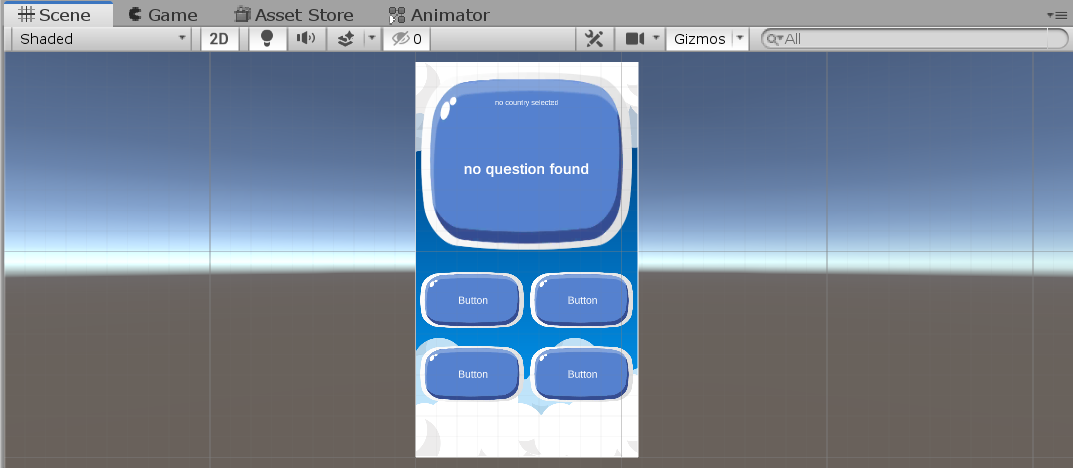
\includegraphics[width=14cm]{quiz_scene.PNG}
\caption{Initialer Status der Quizszene}
\label{fig:quizscene}
\end{figure}

Beim initialen Laden der Szene benötigen wir zuerst die Frage- und Antwortdaten des jeweiligen Landes aus der Datenbank.
Dafür werden erneut Methoden aus der Datenbankschnittstelle, mit dem Übergabeparameter des angeklickten Landes aufgerufen. 
Zuerst laden wir alle Fragen zu dem Land und daraufhin alle Antwortmöglichkeiten zu jeder Frage. 
Die Antwortmöglichkeiten werden an das generierte Frageobjekt angehängt, wodurch eine Liste aus vollständig zusammengesetzten Frageentitäten entsteht.
Diese Liste wird nun innerhalb der Quizszene abgespeichert und kann jetzt, wie im vorher beschriebenen Informationsteil, zum Befüllen der Szene genutzt werden.

Hierfür wird ein C\#-Script benötigt, welches das Verhalten der gesamten Quizszene kontrolliert.
Dieses liegt als eigenes GameObject innerhalb der Szene vor und hält Referenzen auf die in der Szene befindlichen GameObjects.
Es werden die Folgenden benötigt: Der Fragetext, der Text des aktuellen Landes und die vier Buttons der Auswahlmöglichkeiten.
Diese sind alle Objekte die zum Laden eines Quiz nötig sind.

Nun wird Logik benötigt, die über die vorhandenen Fragen iteriert und für jedes Frageobjekt die UI-Texte neu befüllt. Das geschieht innerhalb einer Methode im Script, welche für jede Frage erneut aufgerufen wird. 
Mittels einer Zählervariable weiß sie, welche Frage gerade aktiv ist und befüllt die Szenenoberfläche mit deren Daten.
Hierfür sind die referenzierten GameObjects notwendig, mithilfe derer die Platzhaltertexte überschrieben werden können. 

Damit sich die Reihenfolge der Fragen und die der Antwortmöglichkeiten nicht bei jedem Quizdurchlauf wiederholt, werden sie vorher gemischt. 
Nun müssen wir den Buttons noch \textquote{onClick}-Funktionalität geben. 
Ist eine Antwortmöglichkeit mit dem Flag für \textquote{isCorrectAnswer} versehen, zählt ihr \textquote{onClickListener} einen weiteren Zähler hoch, welcher die korrekten Beantwortungen zählt und ruft anschließend die Initialisierung der nächsten Frage auf. 
Falls nicht, bleibt dieser Zähler gleich und es wird ebenfalls die nächste Frage geladen.

Nach Beantwortung aller Fragen, sollte die erstgenannte Zählervariable der Anzahl an Fragen entsprechen.
Dies dient als Abbruchbedingung des rekursiven Methodenaufrufs zum Laden einer Frage.
Nun wird ausgewertet ob der Nutzer alles richtig beantwortet hat und dementsprechend ein positiver oder ein negativer Feedback-Bildschirm angezeigt.
Dieser informiert darüber ob das Quiz bestanden wurde, zeigt jedoch nicht explizit bei welchen Fragen es nicht geklappt hat.
Von hieraus gelangt man nun durch einen Button wieder zurück zur Kameraansicht der AR-Szene.
\chapter{Fazit}\label{ch:fazit}

% remove if not needed
\appendix
\chapter{Anhang}\label{app:anhang}
\section{Steckbriefe der Personas}\label{persona}
Im Folgenden sind die Steckbriefe der Personas Thorsten und Mark zu sehen. Was für einen Zweck diese erfüllen, wird in Abschnitt \ref{inhaltliche_anforderungen} erklärt.

\begin{figure}[!htb]
\minipage{0.48\textwidth}
  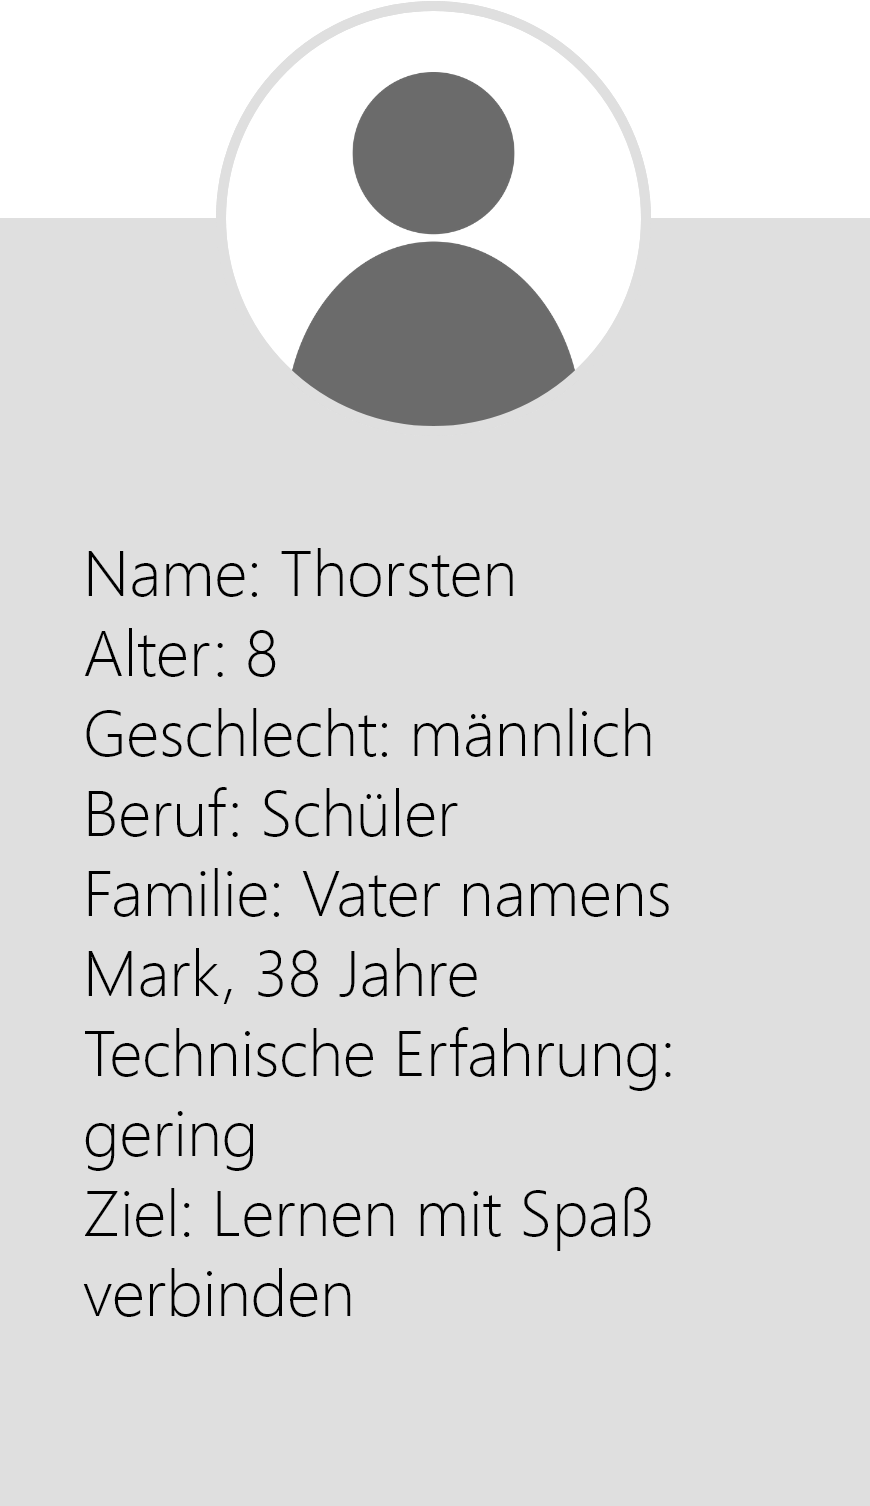
\includegraphics[width=\linewidth]{Persona_1.png}
  \caption{Steckbrief von Thorsten}\label{fig:persona_thorsten}
\endminipage\hfill
\minipage{0.48\textwidth}
  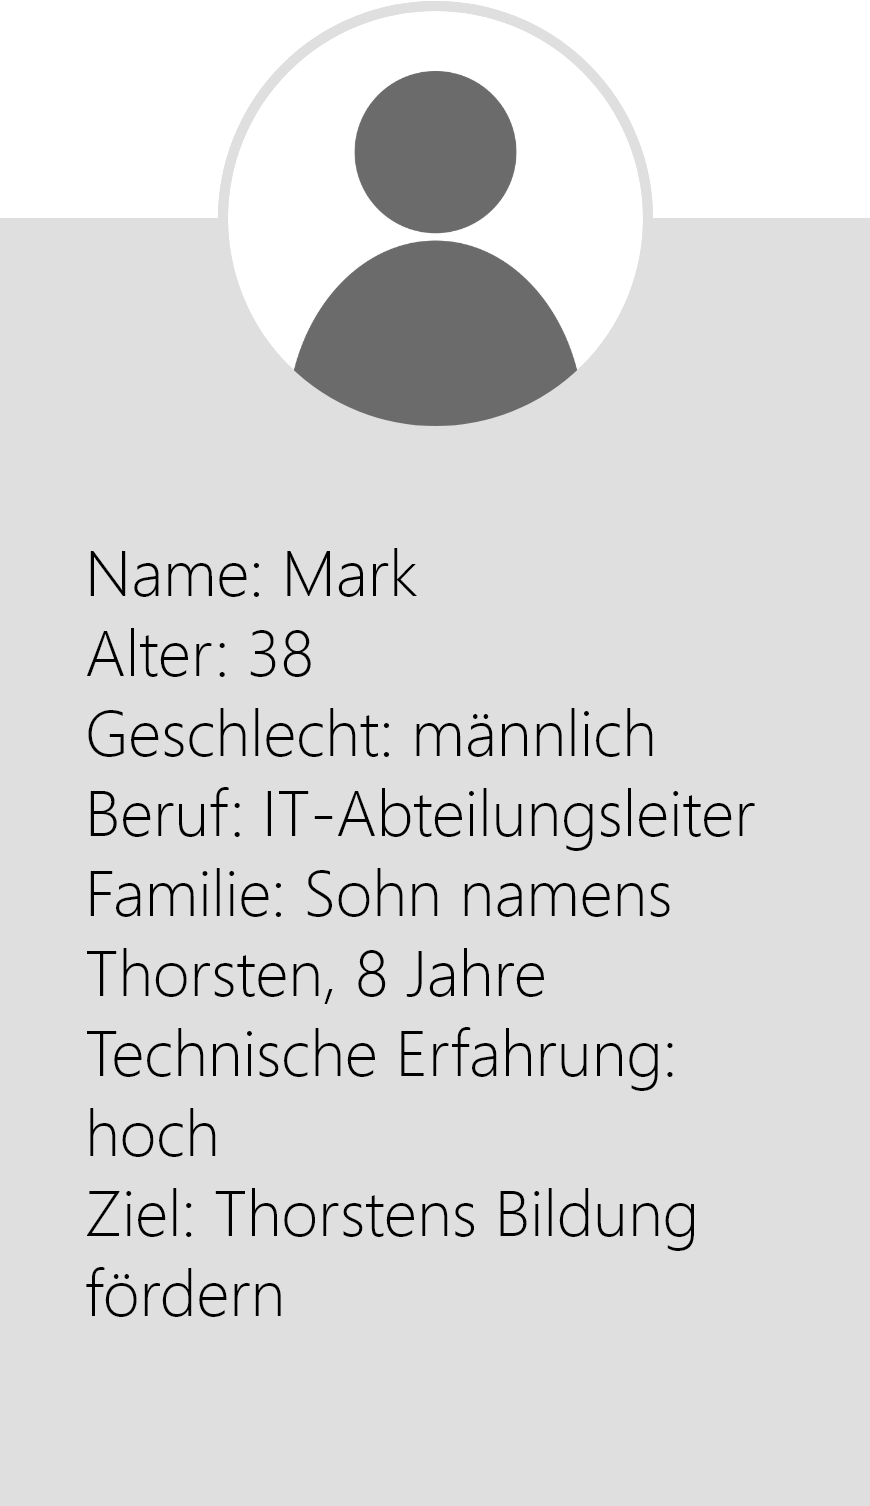
\includegraphics[width=\linewidth]{Persona_2.png}
  \caption{Steckbrief von Mark}\label{fig:persona_mark}
\endminipage\hfill
\end{figure}

\section{Verwendete 3D Objekte}
Die für das Projekt verwendeten 3D Objekte werden im Folgenden mit ihrem zugehörigen Kontinent dargestellt. Diese entstammen verschiedenen Internetquellen, die in Abschnitt \ref{verwendung_3d_objekte} aufgeführt sind.

\begin{figure}[!htb]
\minipage{0.48\textwidth}
  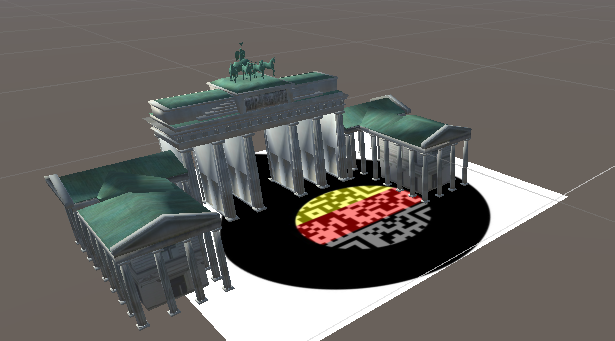
\includegraphics[width=\linewidth]{Deutschland.png}
  \caption{3D Objekt von Deutschland (Europa)}\label{fig:deutschland}
\endminipage\hfill
\minipage{0.48\textwidth}
  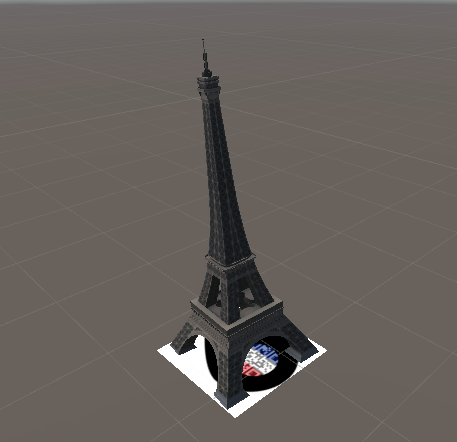
\includegraphics[width=\linewidth]{Frankreich.png}
  \caption{3D Objekt von Frankreich (Europa)}\label{fig:frankreich}
\endminipage\hfill
\end{figure}

\begin{figure}[!htb]
\minipage{0.48\textwidth}
  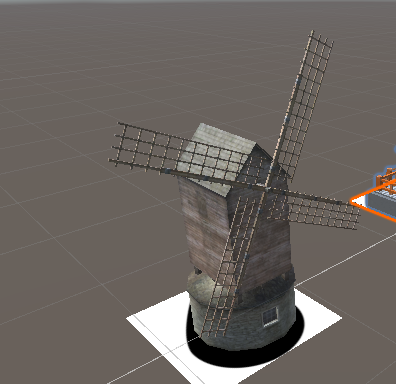
\includegraphics[width=\linewidth]{Niederlande.png}
  \caption{3D Objekt von den Niederlanden (Europa)}\label{fig:niederlande}
\endminipage\hfill
\minipage{0.48\textwidth}
  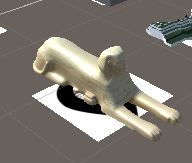
\includegraphics[width=\linewidth]{Aegypten.png}
  \caption{3D Objekt von Ägypten (Afrika)}\label{fig:aegypten}
\endminipage\hfill
\end{figure}

\begin{figure}[!htb]
\minipage{0.48\textwidth}
  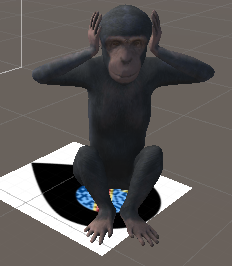
\includegraphics[width=\linewidth]{Kongo.png}
  \caption{3D Objekt vom Kongo (Afrika)}\label{fig:kongo}
\endminipage\hfill
\minipage{0.48\textwidth}
  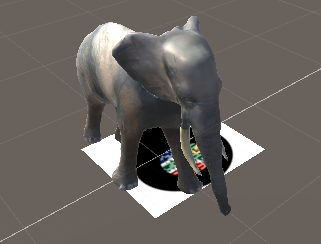
\includegraphics[width=\linewidth]{Suedafrika.png}
  \caption{3D Objekt von Südafrika (Afrika)}\label{fig:suedafrika}
\endminipage\hfill
\end{figure}

\begin{figure}[!htb]
\minipage{0.48\textwidth}
  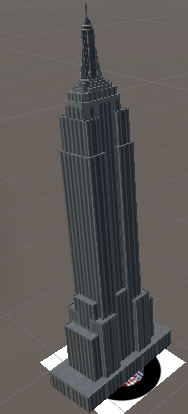
\includegraphics[width=\linewidth]{USA.png}
  \caption{3D Objekt von den USA (Nordamerika)}\label{fig:usa}
\endminipage\hfill
\minipage{0.48\textwidth}
  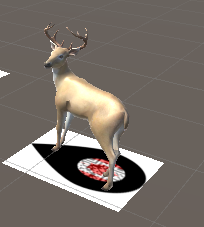
\includegraphics[width=\linewidth]{Kanada.png}
  \caption{3D Objekt von Kanada (Nordamerika)}\label{fig:kanada}
\endminipage\hfill
\end{figure}

\begin{figure}[!htb]
\minipage{0.48\textwidth}
  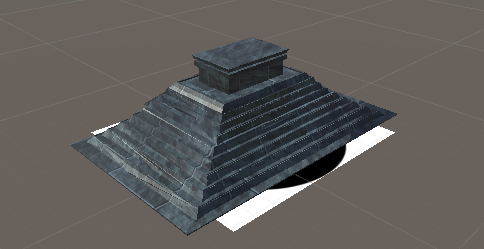
\includegraphics[width=\linewidth]{Mexiko.png}
  \caption{3D Objekt von Mexiko (Nordamerika)}\label{fig:mexiko}
\endminipage\hfill
\minipage{0.48\textwidth}
  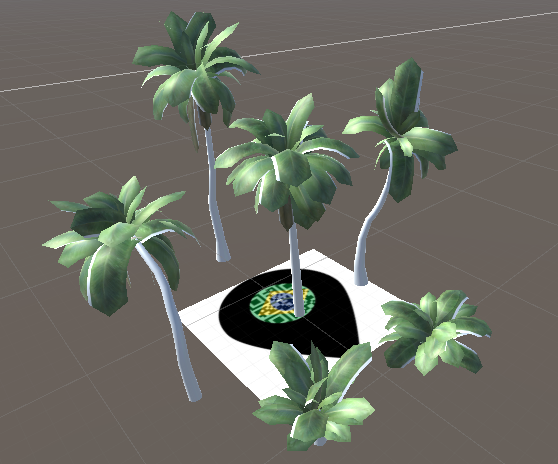
\includegraphics[width=\linewidth]{Brasilien.png}
  \caption{3D Objekt von Brasilien (Südamerika)}\label{fig:brasilien}
\endminipage\hfill
\end{figure}

\begin{figure}[!htb]
\minipage{0.48\textwidth}
  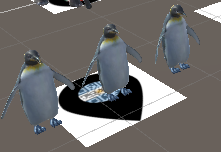
\includegraphics[width=\linewidth]{Argentinien.png}
  \caption{3D Objekt von Argentinien (Südamerika)}\label{fig:argentinien}
\endminipage\hfill
\minipage{0.48\textwidth}
  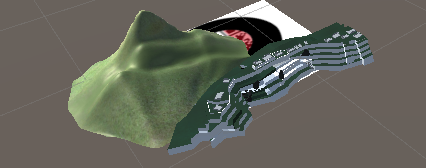
\includegraphics[width=\linewidth]{Peru.png}
  \caption{3D Objekt von Peru (Südamerika)}\label{fig:peru}
\endminipage\hfill
\end{figure}

\begin{figure}[!htb]
\minipage{0.48\textwidth}
  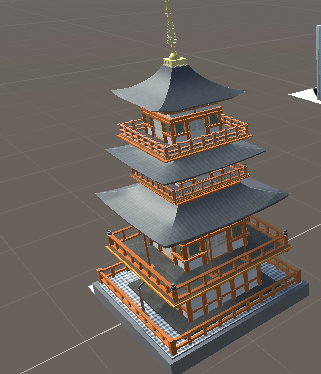
\includegraphics[width=\linewidth]{Japan.png}
  \caption{3D Objekt von Japan (Asien)}\label{fig:japan}
\endminipage\hfill
\minipage{0.48\textwidth}
  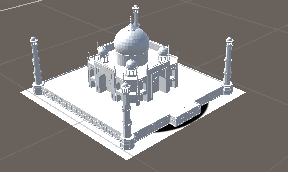
\includegraphics[width=\linewidth]{Indien.png}
  \caption{3D Objekt von Indien (Asien)}\label{fig:indien}
\endminipage\hfill
\end{figure}

\begin{figure}[!htb]
\minipage{0.48\textwidth}
  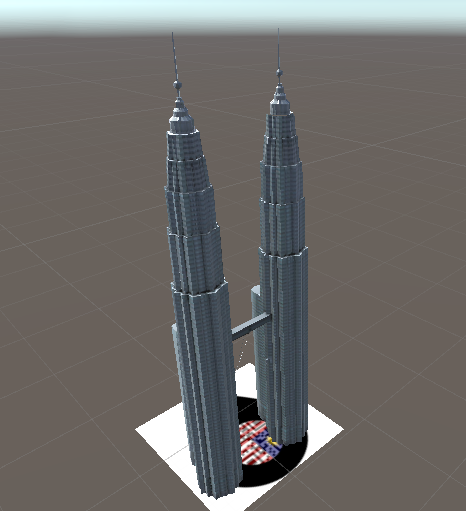
\includegraphics[width=\linewidth]{Malaysia.png}
  \caption{3D Objekt von Malaysia (Asien)}\label{fig:malaysia}
\endminipage\hfill
\end{figure}



\backmatter
\listoffigures
\cleardoublepage

\listoftables
\cleardoublepage

\cleardoublepage

\bibliographystyle{plain}
\bibliography{refs}

\end{document}
